\documentclass[12pt]{article}
\usepackage[utf8]{inputenc}

\usepackage{style}

\title{Decoupled Solution for Composite Sparse-plus-Smooth Inverse Problems}
\author{Adrian Jarret, Julien Fageot}
\date{}

\begin{document}

\maketitle

\begin{abstract}
    We consider composite linear inverse problems where the signal to recover is modeled as a sum of two functions. 
    We study a variational framework formulated as an optimization problem over the pairs of components using two regularization terms, each of them acting on a different part of the solution.
    The specificity of our work is to study the case where one component is regularized with an atomic norm over a Banach space, which is known to promote sparse reconstruction, while the other is regularized with a quadratic norm over a Hilbert space, which promotes smooth solution.

    We show how this composite optimization problem can be reduced to an optimization problem over the Banach space component only up to a linear problem.
    This reveals a decoupling between the two components, allowing for a new composite representer theorem.
    It naturally induces a decoupled numerical procedure to solve the composite optimization problem.

    We exemplify our main result with a composite deconvolution problem of Dirac recovery over a smooth background. In this setting, we illustrate the relevance of a composite model and show a significant temporal gain on signal reconstruction, which results from our decoupled algorithmic approach.

    % \ad{To improve: } This reveals how the joint optimization is made, allows for a new characterization of the extreme point solutions (representer theorem).
    % We exemplify our main results over composite linear inverse problems with Dirac recovery among a smooth signal from Fourier measurements. In this setting,
    % we illustrate how our main theoretical fact can lead to accelerate algorithmic methods for composite inverse problems.
\end{abstract}

\noindent{\it Keywords\/}: Sparse reconstruction, composite model, continuous-domain recovery, functional inverse problems. 

    \ad{
    Remaining todo's:
    \begin{itemize}
        \item \textcolor{red}{Consistency of capitals in the titles.}
        \item check the ad comments
        \item in section~\ref{sec:application} check if I should use $\R$ or $\mathcal{X}$.
        % \item \ju{Unify biblio (eg. T. Debarre vs Thomas Debarre)} -> Seems ok with using bibliographystyle vancouver.
        \item Position of the figures in the document.
        % \item Make new figures with the RKHS model and adapt the text with the new parameters' values.
        \item Import changes from the thesis manuscript.
        \item Check consistency with the journal rules: figure and table no abbreviated.
        \item Use $:=$ for the definitions.
        % \item \textcolor{gray}{Fix the size of the graduations on the plots, and graduations from 0 to 1 instead of 0 to 800 in figures~\ref{fig:simple:blasso-conv}, \ref{fig:simple:bg}, \ref{fig:simple:fg-merged}.}
        % \item \textcolor{gray}{Make reference to Pyxu somewhere.}
        % \item \textcolor{gray}{Do once again all the plots}
        % \item \textcolor{gray}{run the time benchmark and do figures 9 and 10 (time comparisons)}
        % \item \textcolor{gray}{analysis of the last section}
        % \item \textcolor{gray}{homogenize sparse plus smooth or sparse-plus-smooth (also check if italic or not)}
        % \item \textcolor{gray}{Homogenize the hyphen in words like non-something (non-linear vs nonlinear, subcomponent, subproblem).}
        % \item \textcolor{gray}{check if the matrix M is defined in bold or not, consistency of the notation.}
        % \item \textcolor{gray}{check consistency of notation of exponential: $\exp$ or $e^{\dots}$}
        % \item \textcolor{gray}{Regarding bibliography: extract only relevant references and check the arxiv to see if they have been published.}
        % \item \textcolor{gray}{capitals on figures, Sectin, etc... See journal guidelines.}
        % \item \textcolor{gray}{Refer to appendix \ref{app:calculation} somewhere.}
    \end{itemize}
    }
    
\section{Introduction}
    % \ad{\begin{itemize}
    %     \item Elementary computations but cool results
    %     \item Both theoretical and practical contributions: analysis of the solution set and decoupling for numerical solving 
    % \end{itemize}
    % }
    % \noindent\ad{
    % For sure, the article has to present the decoupling result for abstract Banach + Hilbert composite reconstruction.}
    
    % \noindent\ad{
    % Then, different stories are to be considered:
    % \begin{itemize}
    %     \item More oriented toward applications: many consider a RA example, or as Martin suggested more detailed on the quality of the reconstruction.
    %     \item Possible study of the influence of the regularization parameters.
    %     \item More theory-oriented, considering various cases of composite reconstruction:
    %     \begin{itemize}
    %         \item Sparse pline reconstruction with nullspace 
    %         \item Smooth spline reconstruciton with nullspace as well (weird constraint on the null space, could be investigated further)
    %         \item Composite by design, with potionally a regularization operator on the sparse component (comes for free)
    %         \item Composite by design, with regularization operator on the smooth component as well (not sure it works though)
    %     \end{itemize}
    % \end{itemize}
    % }

    \subsection{Composite Linear Inverse Problems}
    
    We study linear inverse problems where the goal is to recover a signal $s^\dagger$ from a finite number of possibly noisy linear measurements $\bm{y} \approx \bm{\Phi}(s^\dagger)$. 
    The inverse problem is called composite if the signal to reconstruct is modeled as a sum of several subcomponents. We consider the case where $s^\dagger$ is the sum of two terms
    \begin{equation}
        s^\dagger = s_1^\dagger + s_2^\dagger
        \label{eq:summodel}        
    \end{equation}
    with different characteristics.
    Such a framework can be used for instance to model signals which contain mixed-types information, such as background and foreground in imaging. A concrete example of composite-type signal is provided in figure~\ref{fig:gleam-sky} with an image of the sky from radio observations, containing both precisely-localized point sources (stars) and diffuse emissions (nebulae) \cite{hurley-walker2017}.
    Our goal is to approximately recover not only $s^\dagger$ but also the subcomponents $s_1^\dagger$ and $s_2^\dagger$ from the observations $\bm{y}$.
    % Such a structure could be interesting for instance for modeling astronomical signals, as we can see in figure~\ref{fig:gleam-sky} in which the image to recover contains both slowly varying features and sparse and precisely-localized point sources \cite{hurley-walker2017}.

    \begin{figure}[t]
        \centering
        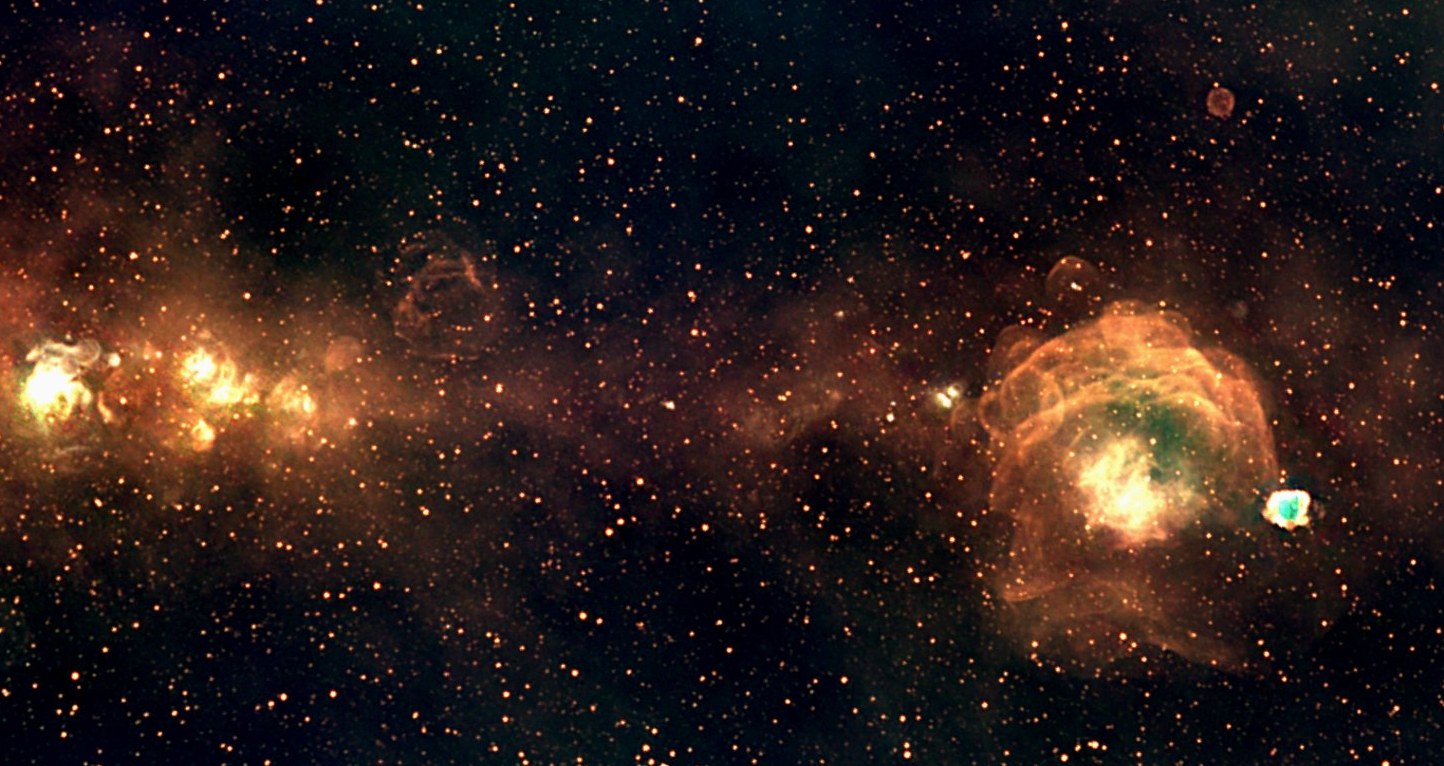
\includegraphics[width=0.8\linewidth]{figures/gleam9h37m15.21s-50deg25min03.1sec.png}
        \caption{Observation of the radio sky at coordinates from the GLEAM survey accessible at \href{https://gleamoscope.icrar.org/gleamoscope/trunk/src/}{gleamoscope.icrar.org}, J2000 coordinates (9h37min15.21s, 50\textdegree25'03.1'').}
        \label{fig:gleam-sky}
    \end{figure}
    
    
    The inverse problem $\bm{y} \approx \bm{\Phi}(s_1^\dagger + s_2^\dagger)$ is generally ill-posed. First, the data are typically insufficient to reconstruct the total information of the original signal: many signals can explain the observation vector $\bm{y}$. Second, the observation vector $\bm{y}$ is often a noisy version of the measurement vector $\bm{\Phi}(s^\dagger)$. Third, the search for the subcomponents comes with an additional difficulty since it requires to separate the sources explaining adequately the observations.

    %Motivation for this composite IP model, examples
    Various classical signal recovery applications are based on a composite model for linear inverse problems.
    % STD, Aujol 2006, Guennec 2024
    For instance, structure-texture decomposition in images corresponds to a simple inverse problem (no forward operator) for which numerous composite models exist \cite{aujol2006std,guennec2024std}.
    % % Foregournd/background separation (Bouwmans for a review), theoretic guarantees for composite sparse plus low rank problem with Tanner.
    % A composite \emph{low-rank plus sparse} model is also classically used for background-foreground separation in images \cite{bouwmans2017decomposition}, for which theoretic reconstruction guarantees have been derived with a compressed sensing analysis \cite{tanner2023composite}.
    % % Background removal techniques (see Vasiliki Colorme)
    % \ad{Choose one of the two next sentences.} Other simpler composite models have been proposed to perform background removal for deconvolution in microscopy. 
    % Background removal has also been studied with other different models, in particular for deconvolution in microscopy \cite{debarnot2020learning,stergiopoulou2022colorme}.
    %% Better version that combines both sentences
    We can also refer to background-foreground separation in images, which usually relies on composite models. They include \emph{sparse-plus-smooth} models, for instance used for deconvolution imaging in microscopy \cite{debarnot2020learning,stergiopoulou2022colorme}, or \emph{low-rank-plus-sparse} models for detecting moving objects from a background in video analysis \cite{bouwmans2017decomposition}, for which theoretic reconstruction guarantees exist \cite{tanner2023composite}.
    % Fourier transform + shot noise, appliation to ECG signals
    Composite modeling has also proven relevant for other types of signals than images. In \cite{marziliano2006blsignals}, the authors propose a joint model of high frequency noise and bandlimited signal to perform exact reconstruction based on the theory of finite rate of innovations, with application to compression of ECG.
    % Spectrogram separation
    The separation of bioacoustic signals through their spectrogram is studied in \cite{kreme2024separation}, relying on a composite model of non-stationary components.
    % Potential use cases in astronomical images, composite objects observed


    A classic strategy for solving ill-posed linear inverse problems is to reconstruct the signal as the solution of an optimization problem. We consider composite optimization problems of the form
    \begin{equation} \label{eq:compositepb}
        (s_1^*,s_2^*) \in \underset{(s_1,s_2)}{\arg\min} \ \mathcal{D}(\bm{y}, \bm{\Phi}(s_1 + s_2)) + \mathcal{R}_1 (s_1) + \mathcal{R}_2(s_2),
    \end{equation}
    in which the data-fidelity $\mathcal{D}(\bm{y}, \bm{\Phi}(s_1 + s_2))$ constrains the solution to correspond to the observations and the regularizations $\mathcal{R}_1 (s_1)$ and $\mathcal{R}_2(s_2)$ promotes specific behaviors according to some prior knowledge (see section~\ref{sec:regularizationblabla}). We specifically consider a \emph{sparse-plus-smooth} model where $\mathcal{R}_1$ is a sparsity-promoting regularization while $\mathcal{R}_2$ favors smooth components.

    We make the assumption that the noise corrupting the data is Gaussian, which motivates the choice of a quadratic data fidelity of the form
    \begin{equation*}
        \mathcal{D} (\bm{y}, \Phi(s)) =  \frac{1}{2} \| \bm{y} - \bm{\Phi}(s) \|_2^2.
    \end{equation*}
    This choice is essential to our analysis, enabling us to later identify a quadratic optimization subproblem. 

    % Composite signal models have already received some interest in the signal recovery literature, as they have demonstrated interesting results for various applications. Early works include the decomposition of images in cartoon plus texture \cite{osher2003decomposition,stark2005decomposition,daubechies2005decomposition} and structure plus texture \cite{aujol2006std}, as well as denoising of high frequency signals \cite{marziliano2006blsignals}. 
    % At the same time, a two-variable optimization algorithm was proposed in \cite{mol2004} for generic finite-dimensional composite linear inverse problems.
    % Later works seemed to have converged to this approach based on penalized optimization. The specific case of smooth plus piecewise constant signals was treated in \cite{gholami2013balanced}. Later works on the structure-texture decomposition have focused on improving the reconstructions with refined penalty terms \cite{ono2014std,guennec2024std}. Recently, composite optimization problems have also been applied to microscopy deconvolution \cite{debarnot2020learning} as well as spectrogram separation for acoustic signals \cite{kreme2024separation}.

    % \ad{OLD: Composite optimization problems have also been studied for themselves, with the introduction of specific composite minimization algorithms \cite{mol2004mixed,gholami2013balanced} (general approach for linear inverse problems, smooth plus piecewise constant for Gholami). Recent articles tend to rely on the formal approach of penalized optimization for composite linear inverse problems, with applications to the structure-texture decomposition \cite{ono2014std, guennec2024std} as well as microscopy deconvolution \cite{debarnot2020learning} or even spectrogram separation \cite{kreme2024separation}. }

    % \ad{Various applications of signal recovery problems can be treated using this composite model. Foreground/background recovery and decomposition. make reference to previous applications (see discrete paper, but do not cite it here).}
    % From the application point of view, \eqref{eq:summodel} can be exemplified as follows. Imagine that the signal to reconstruct $s^\dagger$ is an astronomical sky image with two components, the first one being made of localized stars appearing as point sources, and the second one being made of some background whose statistical properties are known, as in figure~\ref{fig:sky}. 
    % The point sources are typically modeled as a sum of 2D Diracs $s_1^\dagger = \sum_k a_k \delta(\cdot - \bm{x}_k)$ while $s_2^\dagger$ can be modeled as the realization of a Gaussian random field. 
    % Then, sparsity-promoting regularization techniques~\cite{Bredies2013inverse} and smooth regularizations techniques~\cite{Berlinet2011reproducing} are known to perform adequately for the recovery of the single components $s_1^\dagger$ and  $s_2^\dagger$, respectively. Going one step further, we mix these techniques to jointly approximately reconstruct the couple $(s_1^\dagger, s_2^\dagger)$. 

    %Our goal is to show how Hilbertian techniques can be added to known ones for Banach spaces in order 
    
    \subsection{From Sparse versus Smooth to Sparse-plus-Smooth Regularization}
    \label{sec:regularizationblabla}

    Consider for a moment the classical single-component version of the optimization problem~\eqref{eq:compositepb}, i.e.,
    \begin{equation} \label{eq:singletpb}
        \underset{s}{\arg\min} \ \mathcal{D}(\bm{y}, \bm{\Phi}(s)) + \mathcal{R} (s)
    \end{equation}
    that aims at solving a non-composite inverse problem.

    In this work, we distinguish two types of regularization for ill-posed inverse problems. Smooth regularization corresponds to the case where the penalty is a quadratic norm over some Hilbert space $\mathcal{H}$, of the typical form 
    \begin{equation*}
        \mathcal{R} (s) = \lambda \| s \|_{\mathcal{H}}^2.
    \end{equation*}
    The name stems from the smoothing effect it has on the solution \cite{Kimeldorf1970}. Early versions include Tikhonov regularization~\cite{tikhonov1963solution}, known as ridge-regression in statistics~\cite{Hoerl1962ridge}. Smooth regularization has been widely used over more than 70 years, with countless applications. %with applications on discrete domain problems as well as recovery in the continuum \ad{ref needed here?}.
    It is strongly connected to the RKHS theory and thus there exist representer theorems that precisely specify the form of the solution~\cite{Scholkopf2001generalized}. Interestingly, these problems are fairly simple to solve as they can be recast into a finite-dimensional formulation, even when the signals $s$ to recover are continuously defined, as for instance with $\mathcal{H} = \ldx$ the space of square integrable functions over a domain $\mathcal{X}$. 
    % Early versions include Tichonov regularization~\cite{tikhonov1963solution}, known as ridge-regression in statistics~\cite{Hoerl1962ridge}. Over a generic Hilbert space, we will refer to it as smooth regularization for its smoothing effect~\cite{Kimeldorf1970}.
    % Smooth regularization has proven to be efficient, it is strongly related to RKHS theory and representer theorems (which specifies the form of the solution of the optimization problem) in this context~\cite{Scholkopf2001generalized}. 

    The second classical form of regularization considered here involves a norm over of Banach space $\mathcal{B}$ expressed as
    \begin{equation*}
        \mathcal{R} (s) = \lambda \| s \|_{\mathcal{B}}.
    \end{equation*}
    We refer to this type of penalties as sparse regularization, as it is used to reconstruct sparse solutions. More precisely, the solutions are expressed as sums of extreme points of the Banach norm unit ball \cite{boyer2019representer,Unser2020}. It is common to use atomic norms for which the extreme points are sparse vectors \cite{chandrasekaran2012convex}.
    The classical finite-dimensional example is the $\ell_1$-norm over Euclidian $n$-spaces \cite{tibshirani1996regression,chen2001atomic}, however the formalism presented hereabove interestingly applies for infinite-dimensional cases, including the sparse spikes recovery case \cite{laville2021sparse} as well as more complex penalties \cite{laville2023a,ambrosio2023,decastro2024}.
    % The topological structure of the search space is more general than the smooth regularization over Hilbert spaces and thus the penalized optimization problems are usually more difficult to solve in practice, the search space being infinite dimensional for continuous-domain problems.
    The Banach space topology is more general than the smooth regularization over Hilbert spaces and thus the penalized optimization problems are more difficult to solve in practice (infinite-dimensional problems, no gradient, etc)
    
    % Atomic norm~\cite{chandrasekaran2012convex}. Example: $\ell_1$. Explain the general principle. \ad{Splines.}

    In this work, we consider the combination of the two above-mentioned penalties, which we refer to as \emph{sparse-plus-smooth} regularization. We focus on problem~\eqref{eq:compositepb} with
        \begin{equation*}
        \mathcal{R}_1 (s_1) = \lambda_1 \| s_1 \|_{\mathcal{B}} \qquad\text{and}\qquad \mathcal{R}_2 (s_2) = \lambda_2 \| s_2 \|_{\mathcal{H}}^2
    \end{equation*}
    for $\lambda_1, \lambda_2 > 0$. This problem has already been studied in \cite{debarre2021continuous} in a general setting, including continuous-domain reconstruction and regularization operators. The authors demonstrated that the solutions of the composite optimization problem indeed behave as expected: the sparse component $s_1$ admits a sparse structure as if it was solution of a non-composite problem, and similarly the component $s_2$ behaves as the solution of a smooth problem. This result has been exemplified in various finite-dimensional application cases, using sparse-plus-smooth optimization problems with discrete vector components, see \cite{mol2004,gholami2013balanced,debarnot2020learning}. In the discrete setting, it is possible to decouple the resolution of the composite optimization problem: the sparse component can be directly identified with a Banach-penalized problem and the Hilbert component is unique and deduced afterward. The requirements for such a decoupling to take place are presented in \cite{jarret2024decoupled}, considering the general case in which operators are involved within the regularization terms.

    % \ad{Should maybe put more emphasis on the continuun.}
    % \ju{Agreed. It could list possible application frameworks when people use atomic norms in the continuum (Romain Petit, Shayan sur la Schatten norm, l'ancien collègue de Vasi qui bosse sur les courbes comme atomes).} \ad{Good point, done!}

    % \ju{Possible emphasis: algorithmic consequences for all those applications. Many $ell_1$ algo does not apply to $ell_1 + ell_2$ and thanks to our work, now they do up to a linear subproblem. It could be the occasion to quickly refer to those algorithms, such as FW.} \ad{I don't think that is the case. If an algorithm solves a l1 penalized problem, it can solve a composite l1 + l2 problem as the l2 term is differentiable.}

    \subsection{Contributions and Outline}

    Our main contribution is to identify a new way of conceiving the optimization problem \eqref{eq:compositepb} by decoupling its resolution, extending the result of \cite{jarret2024decoupled} to general Banach and Hilbert spaces. More precisely, we show that the composite optimization problem~\eqref{eq:compositepb} can be reduced to two subproblems. The first one is brought back to the Banach space and directly identifies the sparse component, while the second one is a quadratic optimization problem that admits an explicit solution. We obtain a more precise composite representer theorem than existing results and identify in particular the smooth component in closed form as a function of the vector of measurements of the sparse component.

    % We deduce some important algorithmic consequences in the study of specific optimization problems with the case of finite-dimensional inverse problems (regularization norms $\| \cdot \|_1$ and $\|\cdot \|_2$).

    We illustrate the decoupling mechanism on a composite deconvolution problem inspired from microscopy imaging.
    Empirically, we demonstrate in simulations the relevance of using a composite model over a single-component approach for problems involving a smooth background. We also show a significant temporal gain from the use of algorithms exploiting the decoupling of the initial problem compared to the standard approach based on the representer theorem of \cite{debarre2021continuous}. 

    % \section{Related Works}

    % Une section sur le related works.
    % Histoire de Tychonov et conséquence.
    % Histoire de sparsité. Compressed sensing, Sparse statistical learning, etc.

    % Old name: \sout{Smooth versus Sparse} Representer Theorems \ad{for Single Component Problems}}

%%%%%%%%%%%%%%%%%%%%%%%%%%%%%%%%%%%%%%%%%%%%%%%%%%%%%%%%%%%%%%
%%%%%  SECTION 2
%%%%%%%%%%%%%%%%%%%%%%%%%%%%%%%%%%%%%%%%%%%%%%%%%%%%%%%%%%%%%%
\section{Representer Theorems for Single-Component Problems}

    % Named after the regularization. Introduction of notations. Known results.
    As they will be useful later on, we recall here the classical representer theorems that characterize the solutions of single-component optimization problems, along with the relevant topological structures on the search spaces involved. In particular, smooth regularization can be formulated over regular Hilbert spaces while a more precise description of the topology of Banach spaces is needed for sparse regularization. 

    % \subsection{Mathematical Background}
    % \label{sec:mathsbackground}
    
    \subsection{Smooth Regularization of Inverse Problems}

    \ad{We assume the search space $\mathcal{H}$ to be a Hilbert space with Hilbertian norm $s \mapsto \| s \|_\mathcal{H} = \sqrt{\langle s, s \rangle_{\mathcal{H}}}$. By the Riesz representer theorem, any continuous linear functional $\nu: \cH \to \R$ can be represented as the inner product with an element $\phi_\nu \in \cH$, such that $\nu(f) = \langle \phi_\nu, f \rangle_\cH$ for any $f \in \cH$. The topological dual $\cH'$ is then identified as the search space $\cH$ itself. For $\bm{\Phi}= (\phi_1 ,\ldots , \phi_L) \in \mathcal{H}^L$, we denote
    \begin{equation}
        \bm{\Phi}(s) = \left( \langle \phi_1, s \rangle_{\mathcal{H}} , \ldots , \langle \phi_L, s \rangle_{\mathcal{H}} \right). 
        \label{eq:phi-hilbert}
    \end{equation}
    The adjoint of $\bm{\Phi}$ is the only operator $\bm{\Phi}^* : \R^L \rightarrow \mathcal{H}$ which satisfies the equality %\footnotemark{}
    \begin{equation*}
        \langle \phih(s), \bm{y}\rangle_{\R^L} = \langle s, \phih^*(\bm{y})\rangle_\cH,
    \end{equation*}
    for any $s \in \cH$ and $\bm{y}\in\R^L$.
    Its expression is given by $\bm{\Phi}^* (\bm{y}) = \sum_{1 \leq \ell \leq L} y_\ell \phi_\ell$.
    We also consider the Gram matrix $\mathrm{G} = \bm{\Phi} \bm{\Phi}^* \in \R^{L\times L}$ whose entries are given by $G[k,\ell] = \langle \phi_k , \phi_\ell\rangle_{\mathcal{H}}$.}
    % \footnotetext{\ad{The definition of the adjoint operator depends on the inner product $\langle \cdot, \cdot \rangle_\cH$ used on $\cH$. The explicit expression of $\phih^*$ needs to be determined with a particular attention when the choice of this inner product is not canonical. This idea is discussed in \cite{unser2021unifying}, considering the more general concept of \emph{duality mappings} and \emph{conjugate pairs}.}

    % We assume the search space $\mathcal{H}$ to be a Hilbert space with Hilbertian norm $s \mapsto \| s \|_\mathcal{H} = \sqrt{\langle s, s \rangle_{\mathcal{H}}}$. The topological dual of $\mathcal{H}$ is made of functionals $s \mapsto \langle \phi, s \rangle_{\mathcal{H}}$ with $\phi \in \mathcal{H}$.
    % For $\bm{\Phi}= (\phi_1 ,\ldots , \phi_L) \in \mathcal{H}^L$, we denote
    % \begin{equation}
    %     \bm{\Phi}(s) = \left( \langle \phi_1, s \rangle_{\mathcal{H}} , \ldots , \langle \phi_L, s \rangle_{\mathcal{H}} \right). 
    %     \label{eq:phi-hilbert}
    % \end{equation}
    % The adjoint of $\bm{\Phi}$ is the operator $\bm{\Phi}^* : \R^L \rightarrow \mathcal{H}$ such that $\bm{\Phi}^* (\bm{y}) = \sum_{1 \leq \ell \leq L} y_\ell \phi^*_\ell$. Then, $\mathrm{G} = \bm{\Phi} \bm{\Phi}^* \in \R^{L\times L}$ is the Gram matrix whose entries are $G[k,\ell] = \langle \phi_k , \phi_\ell\rangle_{\mathcal{H}}$. 
    
   Proposition \ref{prop:hilbertRT} hereafter is a classical result for quadratic optimization over Hilbert spaces. Significantly more general formulations can be found in~\cite{Scholkopf2001generalized} but we restrict here to the case which is relevant for our purpose. We follow the exposition of~\cite[Theorem~7]{caponera2021nonparametric}, which is based on \cite[Section~3.2]{Unser2020}. 

    \begin{proposition}[Representer Theorem on Hilbert spaces]
    \label{prop:hilbertRT}
    Let $\bm{y}\in \R^L$, $\bm{\Phi}= (\phi_1 ,\ldots , \phi_L) \in \mathcal{H}^L$, and $\lambda > 0$. Given that the measurement functionals $\phi_1, \dots, \phi_L$ are linearly independent, the optimization problem 
    \begin{equation} \label{eq:hibertpb}
        \inf_{s \in \mathcal{H}} \frac{1}{2} \| \bm{y} - \bm{\Phi}(s) \|_2^2 + \frac{\lambda}{2} \| s \|_{\mathcal{H}}^2
    \end{equation}
    admits a unique solution $\hfh \in \mathcal{H}$ which is given by
    \begin{equation} \label{eq:widehathilb}
        \hfh  = \bm{\Phi}^* ( \bm{\Phi} \bm{\Phi}^* + \lambda \mathbf{I}_L)^{-1} \bm{y}.
    \end{equation}
    \end{proposition}
    % \ad{This is okay but hides the difficulty: if the inner product on $\mathcal{H}$ is not canonical $\mathrm{L}_2$ then the adjoint of $\mathbf{\Phi}$ is actually quite tricky to determine and involves the Riesz map of $\mathcal{H}$. The proper reference in this scenario is from \cite[Section~3.2]{Unser2020}.}
    
    \noindent In other terms, Proposition~\ref{prop:hilbertRT} states that the solution set of ~\eqref{eq:hibertpb} is 
    \begin{equation}
        \mathcal{U} (\lambda) := \{ \bm{\Phi}^* ( \bm{\Phi} \bm{\Phi}^* + \lambda \mathbf{I}_L)^{-1} \bm{y}\}.
    \end{equation}
    The existence and uniqueness of the solution of \eqref{eq:hibertpb} follows from the the fact that the functional of \eqref{eq:hibertpb} is continuous and strongly convex due to the quadratic regularization.
    % \ad{We should remove the next sentence I think.}
    The function $ \hfh $ is in the span of the functionals $\phi_\ell$ since \eqref{eq:widehathilb} can be reinterpreted as 
    \begin{equation*}
    \hfh  = \sum_{1 \leq \ell \leq L} \alpha_\ell \phi_\ell \quad \text{where} \quad \bm{\alpha} = ( \bm{\Phi} \bm{\Phi}^* + \lambda \mathbf{I}_L)^{-1} \bm{y} \in \R^L. 
    \end{equation*}

    % \ad{The function $ \hfh $ can be reinterpreted as
    % \begin{equation*}
    % \hfh  = \sum_{1 \leq \ell \leq L} \alpha_\ell \phi_\ell^* \quad \text{with} \quad \bm{\alpha} = ( \bm{\Phi} \bm{\Phi}^* + \lambda \mathbf{I}_L)^{-1} \bm{y} \in \R^L,
    % \end{equation*}
    % in which the ....}
    
    
    \subsection{Sparse Regularization of Inverse Problems}

    The norms responsible for promoting sparsity do not stem from any inner product. The classical framework instead considers the search space being a generic non-reflexive Banach space $\mathcal{B}$ and assumes the existence of a predual space \cite{unser2021unifying}.
    We fix two Banach spaces $( \mathcal{A}, \| \cdot \|_{\mathcal{A}})$ and $( \mathcal{B}, \| \cdot \|_{\mathcal{B}})$ such that $\mathcal{B} = \mathcal{A}'$ is the topological dual of $\mathcal{A}$ and $\| \cdot \|_{\mathcal{B}}$ is the dual norm 
    \begin{equation*}
        \| s \|_{\mathcal{B}} = \sup_{\|g \|_{\mathcal{A}}=1} \langle g, s \rangle_{\mathcal{A}\times\mathcal{B}}, 
    \end{equation*}
    \ad{where the \emph{dual product} is denoted as $\langle g, s \rangle_{\mathcal{A}\times\mathcal{B}} = s(g)$.}
    This assumption implies that $\mathcal{B}$ can be endowed with the weak*-topology inherited from $\mathcal{A}$. We say that the sequence $(s_n)_{n\geq 1}$ of elements $s_n \in \mathcal{B}$ converges to $s \in \mathcal{B}$ for the weak*-topology if 
    \begin{equation*}
        \langle g , s_n \rangle_{\mathcal{A}\times\mathcal{B}} \underset{n\rightarrow \infty}{\longrightarrow} \langle g, s \rangle_{\mathcal{A}\times\mathcal{B}} 
    \end{equation*}
    for any $g \in \mathcal{A}$.
    In other terms, $\mathcal{B}$ admits a predual. The Hilbert search space scenario presented in the previous section corresponds to the case $\mathcal{A} = \mathcal{B} = \mathcal{H}$.

    A typical example is the space of Radon measures $(\mathcal{B}, \|\cdot \|_{\mathcal{B}}) = (\mx, \|\cdot \|_{\mathcal{M}})$ over a continuous domain $\mathcal{X}$. Its predual is the Banach space of continuous vanishing functions for the infinite norm $(\mathcal{A}, \|\cdot \|_{\mathcal{A}}) =(\czx, \| \cdot \|_{\infty})$. The Radon measures remarkably contain Dirac impulses, which make them well-suited for continuous-domain sparse recovery. For any $d\in\mathbb{N}^*$, the case $\mathcal{X}=\mathbb{R}^d$ is for instance presented in~\cite{unser2017splines,Unser2020} and the periodic case $\mathcal{X}=\mathbb{T}^d$ is covered by \cite{fageot2020tv}.
    % Typical examples include $(\mathcal{B}, \|\cdot \|_{\mathcal{B}}) = (\ell_1(\Z), \|\cdot \|_{\ell_1})$, whose predual is the Banach space $(\mathcal{A}, \|\cdot \|_{\mathcal{A}}) =(c_0(\Z), \| \cdot \|_{\infty})$ of vanishing sequences for the infinite norm . Some Banach spaces do not enter in this category. For instance, the space $L_1(\R)$ of integrable functions does not admit a predual space~\cite[Theorem 6.3.7]{albiac2006topics} and is therefore excluded from our analysis.

    Without the Hilbert space structure, the measurement operator $\bm{\Phi}= (\phi_1, \ldots, \phi_L)$ is made of measurement functionals $\phi_\ell \in \mathcal{A}$ from the predual space. Then, $\bm{\Phi}$ specifies a linear and weak*-continuous mapping $\bm{\Phi}: \mathcal{A}' =\mathcal{B} \rightarrow \R^L$ via 
    \begin{equation}
        \label{eq:phi-banach}
        \bm{\Phi} (s )= (\langle \phi_\ell, s \rangle_{\mathcal{A}\times\mathcal{B}})_{1\leq \ell \leq L} \in \mathbb{R}^L.
    \end{equation}

    % Interestingly, it is possible to extend Proposition~\ref{prop:hilbertRT} to this more general setting.
    In this more general setting, the solution set of the optimization problem~\eqref{eq:singletpb} when $\mathcal{R}(s) = \lambda \| s \|_{\mathcal{B}}$ is characterized with another representer theorem in Proposition~\ref{prop:banachRT} hereafter, analogous to Proposition~\ref{prop:hilbertRT} on Hilbert spaces.
    % Interestingly, there exists another representer theorem which plays to counterpart of Proposition~\ref{prop:hilbertRT} in this more general setting.
    % CHANGE ORDER OF THE SENTENCES.
    The specific case of $\lVert \cdot \rVert_\mathcal{B}$ being the $\ell_1$-norm or its functional generalization is studied in~\cite{Fisher1975,Unser2016representer,unser2017splines,bredies2020sparsity}, and some even more general settings are studied in~\cite{boyer2019representer,unser2019native}.
    % Hereafter, Proposition~\ref{prop:banachRT} recalls this result.


    
    % The Banach space generalization of Proposition~\ref{prop:hilbertRT} has been considered in the literature for the $\ell_1$-norm and its functional generalization~\cite{Fisher1975,Unser2016representer,unser2017splines,bredies2020sparsity} and in more general settings in~\cite{boyer2019representer,unser2019native}.
    % Let $\bm{\Phi}= (\Phi_1, \ldots, \Phi_L) \in \mathcal{A}^L$. Then, $\bm{\Phi}$ specifies a linear and weak*-continuous mapping $\bm{\Phi}: \mathcal{A}' =\mathcal{B} \rightarrow \R^L$ via 
    % \begin{equation}
    %     \label{eq:phi-banach}
    %     \bm{\Phi} (f )= (\langle \phi_\ell, f \rangle_{\mathcal{A}\times\mathcal{B}})_{1\leq \ell \leq L} \in \mathbb{R}^L.
    % \end{equation}
    % The adjoint of $\bm{\Phi}$ is given by
    % \begin{equation}
    %    \bm{\Phi}^* (\bm{y}) = \sum_{1 \leq \ell \leq L} y_\ell \phi_\ell \in \mathcal{A}
    % \end{equation}
    % for any $\bm{y}\in \R^L$. 
    % Proposition~\ref{prop:banachRT} describes the solution set of the optimization problem~\eqref{eq:singletpb} when $\mathcal{R}(f) = \lambda \| f \|_{\mathcal{B}}$.

    \begin{proposition}{Representer Theorem on Banach spaces}
    \label{prop:banachRT}
     Let $\bm{y}\in \R^L$, $\bm{\Phi}= (\phi_1 ,\ldots , \phi_L) \in \mathcal{A}^L$, and $\lambda > 0$. Then, the optimization problem 
    \begin{equation} \label{eq:banachpb}
        \inf_{s \in \mathcal{B}} \frac{1}{2} \| \bm{y} - \bm{\Phi}(s) \|_2^2 + \lambda \| s \|_{\mathcal{B}}
    \end{equation}
    admits at least a solution and its solution set $\mathcal{V} (\lambda)$ is weak*-compact, convex, and is the closed convex hull of its extreme points. Any extreme point $\hfb$ of $\mathcal{V} (\lambda)$ is such that 
    \begin{equation} \label{eq:widehatbanachextreme}
        \hfb  = \sum_{1 \leq k \leq K} \alpha_k e_k
    \end{equation}
    where $e_k$ are distinct extreme points of the unit ball of $\|\cdot \|_{\mathcal{B}}$,  $\alpha_k \in \mathbb{R}$, and $0 \leq K \leq L$.

    Moreover, for any combination $\bm{y}, \bm{\Phi},\lambda$ there exists a unique vector $\bm{w} = \bm{w}(\bm{y}, \bm{\Phi},\lambda) \in \R^L$ such that
    \begin{equation} \label{eq:zlambda}
        \forall\ \hfb \in \mathcal{V} (\lambda), \quad \bm{\Phi}(\hfb) = \bm{w}.
    \end{equation}
    \end{proposition}
    
    Proposition~\ref{prop:banachRT} combines existence and topological results from~\cite[Proposition 8]{gupta2018continuous} and the extreme point characterization of \cite[Theorem 3.1]{boyer2019representer}.
    %\ad{The link is not obvious to me with Boyer et al.}
    The existence of a common measurement vector $\bm{w}$ for the solutions of \eqref{eq:banachpb} is classical and uses the strict convexity of the $\ell_2$-norm used in the data fidelity. A proof in a slightly different context can be found, for instance, in~\cite[Proposition 7]{debarre2022sparsest}.
    % \ad{Question to myself: Does it still hold with arbitrary Banach norm, such as an atomic norm for instance ? Remark 3.4 from Boyer says so.}

%%%%%%%%%%%%%%%%%%%%%%%%%%%%%%%%%%%%%%%%%%%%%%%%%%%%%%%%%%%%%%
%%%%%  SECTION 3
%%%%%%%%%%%%%%%%%%%%%%%%%%%%%%%%%%%%%%%%%%%%%%%%%%%%%%%%%%%%%% 

\section{Sparse-plus-Smooth Composite Representer Theorem}

    Building on the analysis of the single-component problems, we now turn to the theoretical study of the composite case.

    \subsection{Main theorem}

    \ad{ToDo: Use phih and phib as defined by Julien.}
    Let us recall the composite problem of interest. For $\lambda_1, \lambda_2 > 0$ we write the objective functional as
    \begin{equation}
        \label{eq:composite-optim}
        \mathcal{J}(\fb, \fh) := \frac{1}{2} \| \bm{y} - (\phib (\fb) + \phih (\fh)) \|_2^2  + \lb \| \fb \|_{\mathcal{B}} + \frac{\lh}{2} \| \fh \|_{\mathcal{H}}^2.
    \end{equation}
    \ad{ToDo: Remove sentence on minimum requirement.}
    The measurement operator $\phib$ samples both the sparse and the smooth components hence we have the minimal requirement that $\phib \in (\mathcal{A} \cap \mathcal{H})^L$. The set of pairs of minimizers is defined as
    \begin{equation} \label{eq:argminisback}
        \mathcal{W} (\lb,\lh) := \underset{(\fb,\fh) \in \mathcal{B} \times \mathcal{H}}{\arg\min} \mathcal{J}(\fb, \fh).
    \end{equation}
    We need to define the matrix
    \ad{ToDo: This matrix only involves phih.}
    \begin{equation}
        \label{eq:def-Mphi}
        \mathbf{M}_{\lh} := \frac{1}{\lh} \left(\phih\phih^* + \lh \mathbf{I}_L\right) = \frac{1}{\lh} \left( \langle \phi_k , \phi_\ell \rangle_{\mathcal{H}} + \lh \delta[k - \ell] \right)_{1\leq k, \ell \leq L}.
    \end{equation}
    This matrix is strictly positive definite. It is therefore invertible and admits a square-root matrix.

    Our main result, Theorem~\ref{theo:main} hereafter, reduces the analysis of a composite optimization problem over $\mathcal{B}\times\mathcal{H}$ to a problem over $\mathcal{B}$, hence decoupling the contributions of the two components. The proof is given in Appendix~\ref{app:prooftheo1}.

    \begin{theorem} \label{theo:main}
    \ad{ToDo: Adapt hypothesis on the definition of phi.}
     Let $\bm{y}\in \R^L$, $\lambda_1, \lh > 0$, $\phib \in (\mathcal{A} \cap \mathcal{H})^L$.
     Then, the solution set $\mathcal{W} (\lb,\lh)$
   %  \begin{equation*}
   % \mathcal{W} (\lb,\lh) = \underset{(\fb,\fh) \in \mathcal{B} \times \mathcal{H}}{\arg\min} \| \bm{y} - (\phib (\fb) + \phih (\fh)) \|_2^2  + \lb \| \fb \|_{\mathcal{B}} + \lh \| \fh \|_{\mathcal{H}}^2
   %  \end{equation*}
    is non-empty, convex, and weak*-compact in $\mathcal{B}\times \mathcal{H}$. Moreover, we can write
    \begin{equation}
        \label{eq:decoupling}
        \mathcal{W} (\lb,\lh) = \mathcal{V}(\mathbf{M}_{\lh},\lb) \times \{\hat{f}_2\}
    \end{equation}
    \ad{ToDo: s2 involves phih.}
    with
    \begin{align}
        \mathcal{V}(\mathbf{M}_{\lh},\lb) &= \underset{ \fb \in \mathcal{B}}{\arg\min} \quad \|\mathbf{M}_{\lh}^{-\frac{1}{2}} ( \bm{y} - \phib(\fb)  ) \|_2^2  + \lb \| \fb \|_{\mathcal{B}} , \label{eq:banachpart} \\
        \hfh &=  \frac{1}{\lh}\phih^* \mathbf{M}_{\lh}^{-1} \left(\bm{y} - \bm{w}\right), \label{eq:hilbertpart}
    \end{align}
    where the vector $\bm{w} = \phib ( \hfb)$ is unique and independent of the solution $\hfb \in \mathcal{V}(\mathbf{M}_{\lh},\lb)$. 
    \end{theorem}

    Consequently, known results over $\mathcal{B}$ are directly transferred into $\mathcal{B}\times \mathcal{H}$. We illustrate this principle with the following corollary, expressed as a representer theorem, which characterizes the extreme point solutions of composite inverse problems.

    \begin{corollary}
    From \eqref{eq:banachpart}, we can deduce that the extreme points of $\mathcal{W} (\lb,\lh)$ are of the form 
    \begin{equation} \label{eq:extreme}
        (\hfb , \hfh ) = \left( \sum_{1 \leq k \leq K} \alpha_k e_k , \hfh \right)
    \end{equation}
    where $\alpha_k \neq 0$, $e_k$ are distinct extreme points of the unit ball $\{ \fb \in \mathcal{B}, \ \| \fb \|_{\mathcal{B}} \leq 1\}$, $0 \leq K \leq L$, and $\hfh$ is given by \eqref{eq:hilbertpart}. 
    \end{corollary}

    Theorem~\ref{theo:main} reveals the interests of a composite framework using Banach and Hilbert regularizations. The Banach component is made of extreme points of the unit ball of $\mathcal{B}$
    while the Hilbertian component lives in the finite-dimensional space of the measurement functionals $(\phi_1, \ldots, \phi_L)$. It implies in particular that the general form of an extreme point solution is 
    \begin{equation*}
        \widehat{s} = \hfb + \hfh = \sum_{1 \leq k \leq K} \alpha_k e_k + \sum_{1 \leq \ell \leq L} \beta_\ell \phi_{\ell},
    \end{equation*}
    with $K\leq L$ and where the $e_k$ are distinct extreme points of the unit ball of $\mathcal{B}$. 
    This characterization is particularly relevant for Banach spaces whose extreme points have interesting properties, as is the case for $\ell_1$-norms and their generalizations~\cite{chandrasekaran2012convex}.
    This last equation was already a consequence of~\cite[Theorem 2]{unser2022convex}, but Theorem~\ref{theo:main} specifies the joint properties of the weight vectors $\bm{\alpha}$ and $\bm{\beta}$.

    \begin{remark}[Decoupling of Hilbert-plus-anything]
        We stated Theorem~\ref{theo:main} for Hilbert-plus-Banach optimization but the decoupling readily holds for more general situations. Indeed, the proof only relies on the closed-form expression of the Hilbert component when the other one is fixed.
        It is for instance possible to consider spline reconstruction using $\|\mathrm{L}\cdot\|_\mathcal{B}$ instead of $\|\cdot\|_\mathcal{B}$, with $\mathrm{L}$ a pseudo-differential operator \cite{unser2017splines}.
        When a more general penalty term $\mathcal{R}(\fb)$ is used, the decoupling between the components still holds but the properties that stem from $\mathcal{V}(\mathbf{M}_{\lh}, \lb)$ need to be verified depending on the chosen regularization, see the representer theorems of \cite{boyer2019representer}.

        % Hence, it is possible to replace $\|\cdot\|_\mathcal{B}$ by any penalty term, for instance considering spline reconstruction with $\|\mathrm{L}\cdot\|_\mathcal{B}$ for $\mathrm{L}$ a pseudo-differential operator.
        % % or considering another norm/functional for $\mathcal{R}(f_1)$.
        % When a more general penalty term $\mathcal{R}(f_1)$ is used, the decoupling between the components still holds but the properties that stem from $\mathcal{V}(\mathbf{M}_{\lh}, \lb)$ are not guranteed and need to be verified according to the chosen regularization (representer theorem, uniqueness of measurement vector $\bm{w}$).
    \end{remark}

    \ad{Remove next remark.}
    \begin{remark}[Different measurement operators]
        The data-fidelity term of equation~\eqref{eq:composite-optim} considers that the two components $s_1$ and $s_2$ are measured through the same operator $\phib$. The decoupling of Theorem~\ref{theo:main} still holds if different operators $\phib_1 \in \mathcal{A}^L$ and $\phih_2 \in \mathcal{H}^L$ are considered, each of the applying to a different component. In this case, the expression of the matrix $\mathbf{M}_{\lh}$ needs to be changed accordingly.
    \end{remark}

    \subsection{Maximum regularization parameter for TV-norm}

    Setting the regularization parameters in optimization problems is a notoriously sensitive task. 
    If we consider a single-component problem with a Hilbert penalty, there exists an optimal value of the regularization parameter when the source signal follows a random Gaussian model \cite{Badou}. Beyond this ideal model, finding a relevant value for this parameter is still an open question and many strategies have been proposed in the literature \cite{hansen2000,park2008parameter}. The case of single-component Banach problems is not simpler \cite{deladalle2014sugar,chirinos2024parameter}. 
    However, when an $\ell_1$-norm or total variation norm is considered, the regularization parameter of Banach-penalized problems can be theoretically bounded and we can determine a range of relevant values for $\lambda$. Indeed, there exists a problem-dependent maximum value $\lambda_{\mathrm{max}} > 0$ above which the solution of the optimization is unique and reduced to the null signal. This is a well-known result for LASSO-type problems, both in discrete \cite{tibshirani2013lasso}, \cite[Proposition~II.1]{koulouri2021} and continuous settings \cite[Proposition~10]{debarre2022sparsest}.

    % Given a Gaussian random model on the data/measurements, there exists a theoretic optimal value for the regularization parameter of the single-component optimization problem with an Hilbert penalty \cite{}. This result however does not exist for a generic optimization problem and finding a rule to set the regularization parameter is an active field of research 
    % \ad{Next introductive sentences need to be rephrased. I can mention that some techniques exist. We have more results for Hilbert-type regularization. References: chapter 7 of Rank-Deficient and discrete Ill-posed problems (Hansen), Wahba 1979, also from Hansen ``The L-curve and its use in the numerical treatment of inverse problems'', also see discussion in article from Park, 2017; another recent discusison in ``On learning the optimal regularization parameter in inverse problems'', Rodriguez 2024 -- FInally we have SUGAR paper from Peyré et al, 2014. }
    % For single-component problems, there exists a theoretic optimal value when a Hilbert norm regularization is used \ad{reference needed here}. To the best of our knowledge, such result does not exist for a general Banach norm regularization. 
    % % When Hilbert regularization is considered for a single component problem, it is possible to determine a value that is optimal in the sense of mean square error estimation

    %--------------------

    This result on the maximum value of the regularization parameter can be transferred to composite problems using Theorem~\ref{theo:main}. It reveals an explicit dependence between the two regularization parameters of composite problems, as illustrated in Proposition~\ref{prop:lmax}.

    % In our composite optimization setting, it is possible to rely on such results to also propose an interpretation of the two regularization parameters. Let us consider the classical scenario in which the Banach component is a sparse Radon measure penalized using the associated total-variation norm.
    % Thanks to Theorem~\ref{theo:main}, the regularization paramaters of the composite problem can be interpreted with the same tools when the Banach regularization obeys the same $\ell_1$-like guarantee 
    % we can transfer the same type of guarantee on the regularization parameters of composite problems when the Banach regularization has responds to 

    % we can apply this result to composite problems in which the Banach regularization obeys the same property. Proposition~\ref{prop:lmax} illustrates this transferred property onto the values of the two regularization parameters.
    %--------------------

    \begin{proposition}[Maximum value of $\lambda_1$]
    \label{prop:lmax}
    Let $\mathcal{X}$ be a continuous domain $\mathcal{X}=\mathbb{R}^d$ or $\mathcal{X}=\mathbb{T}^d$ for $d \in \mathbb{N}^*$.

    We consider the composite optimization problem \eqref{eq:argminisback} where $\mathcal{B} = \mathcal{M}(\mathcal{X})$ and $\lVert \cdot \rVert_\mathcal{B} = \lVert \cdot \rVert_\mathcal{M}$. We define
    \begin{equation}
        \label{eq:l1max}
        \begin{split}
        \lambda_{1, \mathrm{max}} &= \lVert \phib^* \mathbf{M}_{\lambda_2}^{-1} \bm{y} \rVert_\infty \\
                & = \lambda_2 \lVert \phib^* \left( \phih \phih^* + \lambda_2 \mathbf{I}_L \right)^{-1} \bm{y} \rVert_\infty.
        \end{split}
    \end{equation}
    For any $\lambda_1 \geq \lambda_{1, \mathrm{max}}$, the solution set for the Banach component is reduced to the singleton zero 
    $$\mathcal{V}(\mathbf{M}_{\lh}, \lb) = \left\{ 0 \right\}$$
    and Problem \eqref{eq:argminisback} is equivalent to a single-component Hilbert problem.
    \end{proposition}

    \begin{proof}
        Problem \eqref{eq:banachpart} is a B-LASSO problem with operator $\mathbf{M}_{\lh}^{-\frac{1}{2}} \phib$ and measurement vector $\mathbf{M}_{\lh}^{-\frac{1}{2}}\bm{y}$, hence the maximum value of the optimization parameter writes as
        \begin{equation*}
            \lambda_{1, \mathrm{max}} = \lVert (\mathbf{M}_{\lh}^{-\frac{1}{2}} \phib)^*  (\mathbf{M}_{\lh}^{-\frac{1}{2}} \bm{y}) \rVert_\infty = \lVert \phib^* (\mathbf{M}_{\lh}^{-\frac{1}{2}})^* \mathbf{M}_{\lh}^{-\frac{1}{2}} \bm{y} \rVert_\infty = \lVert \phib^* \mathbf{M}_{\lambda_2}^{-1} \bm{y} \rVert_\infty,
        \end{equation*}
        using the symmetry of the matrix $\mathbf{M}_{\lambda_2}$.
    \end{proof}

    Equation \eqref{eq:l1max} demonstrates a natural dependence of $\lb$ onto $\lh$. Indeed, the range of relevant values for $\lb$ is $[0, \lambda_{1, \mathrm{max}}]$ which depends on $\lh$. Hence, by first choosing $\lh$ then setting $\lb = \alpha \lambda_{1, \mathrm{max}}$ for $0 < \alpha < 1$ we ensure that the value of the regularization parameters is consistent with the problem. This approach was already proposed and discussed in our previous work on composite problems \cite{jarret2024decoupled}. We illustrate this dependency and how our scaling rule allows to decouple the choice of parameters with a cross table of reconstructions in Appendix~\ref{app:reconstructions}.

    % Benefits of the result: natural scaling of regularization paramter, order of the selection of the parameters. Refernce to this approach is our previous paper \cite{jarret2024decoupled}.

    Additionally, equation \eqref{eq:l1max} provides information on the asymptotic behavior of $\lbm$. When $\lambda_2$ is small, $\lh \mathbf{I}_L$ is negligible compared to $\phih \phih^*$ and so $\lbm$ is proportional to $\lh$. However, for large values of $\lh$, the Gram matrix $\phih \phih^*$ is itself negligible and $\lbm$ tends to $\lVert \mathbf{H}^* \bm{y}\rVert_\infty$. This latter result is consistent with the maximum value of the regularization parameter for the single-component B-LASSO problem.

    % Interesting asymptotic behavior : when $\lambda$ gets very small, $\lambda_1$ needs to be scaled accordingly (regime of linear dependency).

    % \ad{\textbf{Outdated}, how does lambda max compare to the continuous one though?}
    % Note that it is possible to compute the maximum critical value for the regularization parameter based on this equation. We obtain
    % \begin{align*}
    %     \lambda_{1, max} &= \lVert \mathbf{H}^* \mathbf{M}_{\lambda_2}^{-1} \bm{y} \rVert_\infty \\
    %             & = \lambda_2 \lVert \mathbf{H}^* \left( \phih \phih^* + \lambda_2 \mathbf{I}_L \right)^{-1} \bm{y} \rVert_\infty
    % \end{align*}
    % Hence when $\lambda_2 = o(\sigma_{max}^2(\phih))$, $\lambda_{1, max}$ is proportional to $\lh$. Contrarily, when $\lambda_2 \gg \sigma_{max}^2(\phih)$, $\lambda_{1, max} \to \lVert \mathbf{H}^* \bm{y}\rVert_\infty$.

%%%%%%%%%%%%%%%%%%%%%%%%%%%%%%%%%%%%%%%%%%%%%%%%%%%%%%%%%%%%%%
%%%%%  SECTION 3
%%%%%%%%%%%%%%%%%%%%%%%%%%%%%%%%%%%%%%%%%%%%%%%%%%%%%%%%%%%%%%

%!TEX root = main.tex

\section{Application to Super Resolution Deconvolution}
\label{sec:application}

    Deconvolution is a classical imaging inverse problem, appearing in various practical applications such as microscopy, photography or astronomy. It consists in recovering a high resolution image from blurred observations, possibly corrupted by various artifacts (measurement noise, external illumination, etc).
    The presence of background information in the signal to recover, even with a small intensity, significantly deteriorates the quality of traditional sparsity-based single-component reconstruction methods.

    In this section, we illustrate our representer theorem for a deconvolution composite optimization problem. We first emphasize the decoupling in the specific case of \emph{measures-plus-Hilbert} signal before performing actual reconstructions using a grid-based approximation of continuous-domain sparse signals.

    % In this section, we consider a composite signal model and illustrate the benefits of our representer theorem for a deconvolution optimization problem. In particular, composite modeling accurately recovers the unknown signal in situations where single-component problems fail to distinguish foreground from background information. Additionally, using a decoupled numerical procedure reduces the computation time compared to a direct 2-variables approach of the composite optimization problem.

    % The numerical experiments in this section have been implemented with the Python programming language based on the optimization package \texttt{Pyxu} \cite{pyxu-framework}. All the simulations have run on a workstation with 2 CPUs Intel Xeon E5-2680 v3 \@2.5 Ghz, 30 MB cache and 24 threads each. 
    \subsection{Definition of the composite model}
    \label{sec:comp:model}

        % We consider a composite deconvolution inverse problem in which the signal to recover is the sum of a sparse foreground component and a smooth background component.   
        % Such scenario is inspired from Single Molecule Localization Microscopy (SMLM) in which the signal of interest is an image of fluorescent molecules \cite{sage2019smlm}.
        % % The measurement procedure is modeled as a convolution with the point-spread function (PSF) of the microscope.
        % The action of the microscope on the scene is modeled by a convolution with its known point-spread function (PSF).
        % Out-of-focus particles appear more spread-out and fainter than the objects in the focal plan, hence motivating for a composite model with a sparse component to account for the foreground and a smooth one for the background.
        % Moreover, using a continuous signal model is relevant for SMLM as it is possible to reach a resolution below the diffraction limit, relying on the sparse nature of the observed molecules \cite{huang2017super,denoyelle2019sliding,laville2021sparse}.
        
        We consider a scenario inspired from Single Molecule Localization Microscopy (SMLM) in which the signal of interest is an image of fluorescent molecules \cite{sage2019smlm}. Out-of-focus particles appear more spread-out and fainter than the objects in the focal plan, hence motivating for a composite model. Moreover, using a continuous signal model is relevant for SMLM as it is possible to reach a resolution below the diffraction limit, relying on the sparse nature of the observed molecules \cite{huang2017super,denoyelle2019sliding,laville2021sparse}.


        % \subsubsection{Problem definition}
        We first describe a simplified composite inverse problems which mimics the characteristics of SMLM recovery. The measurements $\bm{y}\in\R^L$ are expressed as
        \begin{equation*}
            \bm{y} \approx S \left\{g * (s_1^\dagger + s_2^\dagger)\right\}.
        \end{equation*}
        in which the ground truth signal $s^\dagger := s_1^\dagger + s_2^\dagger$ is the sum of a sparse foreground component $s_1^\dagger \in \mathcal{B}$ and a smooth background component $s_2^\dagger \in \mathcal{H}$. The action of the microscope on the scene is modeled as the convolution with the \emph{point-spread function (PSF)} $g$, before sampling on the grid of observation pixels with the operator $S$.


        \subsubsection{Function spaces}
            For $d \in \mathbb{N}^*$, let $\mathcal{X} = \mathbb{R}^d$ be the continuous domain of the $d$-dimensional signal to recover $s^\dagger$. 

            We consider the classical model of Radon measures $\mathcal{B} = \mx$, in which sparse signals can be represented with Dirac impulses. The \textit{total-variation norm} $\norm{\cdot}_\mathcal{M}$ on $\mx$ is known to promote sparse solutions when used as a regularizer for optimization problems \cite{unser2017splines}. For $\czx$ the space of continuous vanishing functions on $\mathcal{X}$, which is the predual of $\mx$, we recall the dual definition of the total-variation norm
            \begin{equation*}
                \forall m \in \mx, \quad \lVert m \rVert_\mathcal{M} = \underset{\substack{\varphi \in \czx \\ \| \varphi \|_\infty = 1}}{\sup} \int_\mathcal{X} \varphi(x) \mathrm{d}m(x).
            \end{equation*}
            
            % For the smooth background component $s_2$, we consider the Hilbert space of square integrable functions $\mathcal{H} = \ldx$ equipped with the inner product
            % \begin{equation*}
            %     \forall f, h \in \ldx, \quad \langle f, h\rangle_2 = \int_\mathcal{X} f(x) h(x) \mathrm{d}x.
            % \end{equation*}
            % The resulting Hilbert norm over $\ldx$ is noted as $\norm{\cdot}_2$.

            For the smooth background component $s_2$, we consider the Hilbert space $\cH = \cHk$ the RKHS\footnote{\textit{Reproducing Kernel Hilbert Space}.} induced by the Gaussian kernel $k: \cX \times \cX \to \R$, also called \emph{Gaussian radial basis function}, defined as
            \begin{equation*}
                \forall x, y \in \cX, \qquad k(x, y) = g_0(\norm{y - x}) := \frac{1}{(\sqrt{2\pi\sigma_0^2})^d} \exp{ \left({-\frac{\norm{y - x}^2}{2 \sigma_0^2}}\right)},
            \end{equation*}
            for $\sigma_0 > 0$. The kernel $k$ defines an inner product $\langle \cdot, \cdot \rangle_{\cHk}$ and the associated Hilbert norm $\norm{\cdot}_{\cHk}$ on $\cHk$. The formal construction of the RKHS is technical and we refer for instance to \cite[Chapter~10]{wendland2004}. Notably, no direct expression for the inner product  $\langle f, g \rangle_{\cHk}$ is available in the general case of arbitrary $f, g \in \cHk$. This Gaussian RKHS $\cHk$ is a subspace of the square integrable functions $\ldx$, containing the functions with spectral decay dominated by the decay of $k$ (see, e.g., \cite{minh2010} for a more detailed characterization of $\cHk$). We later rely on this property to adjust the intensity of the promoted smoothness and tune the reconstruction with $\sigma_0$.

            Additionally, we assume that the ground truth signals $s_1^\dagger$ and $ s_2^\dagger$ have a compact support, included in the field of view of the microscope. Without loss of generality, we consider this support to be included in the interval $[0, 1]^d$. 


        \subsubsection{Measurement operator}        
            In an optical system, each pixel of the sensor collects part of the light coming from the scene and produces one measurement $y_\ell$. This procedure is classically modeled with a convolution between the PSF of the measurement device $g \in \cHk \cap \czx$ and the observed signal $s = s_1 + s_2$ followed by local integration on a uniform grid \cite{denoyelle2019sliding}. For simplicity, we replace the integration step with a pointwise evaluation of the convolution on the grid.
        
            The sensor is made as a $d$-dimensional uniform grid of $K$ pixels per dimension, leading to $L = K^d$ measurements. The pixel locations are noted as $(x_\ell)_{\ell = 1, \dots, L}$ with $x_\ell \in [0, 1]^d$. For instance, $d=1$ leads to $L=K$ and $x_\ell = {\ell}/({L-1})$ for $\ell \in \{0, \dots, L-1\}$.
        
            % \ad{ToDo: In the current state, the operator Phih is defined as a regular function inner product, which coincides with the definition of the dual product in S' x S. We need to write the components of Phih as inner prodcts in the RKHS, that means identifying representers for the measurements functionals.}
            It leads to the following expression for the two measurement operators of \eqref{eq:composite-optim}. Consider $\ell \in \{1, \dots, L\}$.
            \begin{itemize}
                \item Definition of $\phib$:
            \begin{equation}
                \label{eq:phib-conv}
                \begin{split}
                \forall \fb \in \mx, \qquad \left[\phib(\fb)\right]_\ell &= \left(g*\fb\right)(x_\ell) \\
                &= \int_\cX g(x_\ell - x) \mathrm{d}\fb(x).
            \end{split}
            \end{equation}
            Keeping the notation of equation \eqref{eq:phi-hilbert}, this measurement operator corresponds to the measurement functionals
            $$\phibb_\ell = g(x_\ell - \cdot) \in \czx.$$
                \item Definition of $\phih$:
            \begin{equation}
                \label{eq:phih-conv}
                \begin{split}
                \forall \fh \in \cHk, \qquad\left[\phih(\fh)\right]_\ell &= \left(g*\fh\right)(x_\ell) \\
                &= \int_\cX g(x_\ell - x) \fh(x) \mathrm{d}x.
                \end{split}
            \end{equation}
            However, the identification $\phihh_\ell$ from equation \eqref{eq:phi-banach} is not directly possible due to the absence of the inner product $\langle \cdot, \cdot \rangle_{\cHk}$ and is therefore deferred to Proposition~\ref{prop:phihh}.
            \end{itemize}

            {\color{red}
            \begin{proposition}[Lemma~10 in \cite{Berlinet2011reproducing}]
                \label{prop:phihh}
                For any $\fh \in \cHk$, for $\ell \in \left\{ 1, \dots, L \right\}$, the measurement operator can be written as
                \begin{equation}
                    [\phih(\fh)]_\ell = \langle \phihh_\ell, \fh \rangle_{\cHk}
                    % = \int_\cX g(x_\ell - x) s_2(x) \mathrm{d}x = \int_\cX \phi_\ell(x) s_2(x) \mathrm{d}x
                \end{equation}
                with $\phihh_\ell$ being the convolution
                \begin{equation}
                    \phihh_\ell = g_0 * g(x_\ell - \cdot).
                \end{equation}
            \end{proposition}
            \begin{proof}
                % \ad{ToDo: This is a very classical result but I don't manage to find a good reference. The core idea is as follows.}
                
                % Using the reproducing property, we have:
                % $$\forall \fh \in \cHk, \forall x \in \mathcal{X}, \quad \fh(x) = \langle \fh, k(x, \cdot)\rangle_{\cHk}$$
                % Hence, we can write:
                % \begin{align*}
                %     [\phih(\fh)]_\ell &= \int_\R g(x_\ell - x) \fh(x) \mathrm{d}x \\
                %     & = \int_\R g(x_\ell - x) \langle \fh, k(x, \cdot)\rangle_{\cHk} \mathrm{d}x \\
                %     & = \langle \fh, \int_\R g(x_\ell - x) k(x, \cdot) \mathrm{d}x \rangle_{\cHk} \\
                %     & = \langle \fh, \philk \rangle_{\cHk}.
                % \end{align*}
                % \ad{The inversion between integral and inner product needs to be properly defined and justified, that's why I would like to find a good reference.}

                % \ad{Second proof, simpler.}
                By Riesz representer theorem, for every coordinate  $\ell \in \left\{1, \dots, L \right\}$, there exists an element $\phihh_\ell \in \cHk$ such that for any $\fh \in \cHk$ it holds $[\phih(\fh)]_\ell = \langle \phihh_\ell , \fh \rangle_{\cHk}$. In particular, for $t \in \cX$, using $\fh = k(\cdot, t)$ and the reproducing property, we obtain
                \begin{align*}
                    \forall t \in \cX, \qquad \phihh_\ell(t)
                    &= \langle \phihh_\ell, k(\cdot, t) \rangle_{\cHk} = [\phih(k(\cdot, t))]_\ell \\
                    & = \int_\cX g(x_\ell - x) k(x, t) \mathrm{d}x = \int_\cX g(x_\ell - x) g_0(t - x) \mathrm{d}x \\
                    & = (g(x_\ell - \cdot) * g_0)(t).
                \end{align*}   
            \end{proof}
            }
            
            We consider the simplistic model of the PSF being an isotropic Gaussian function of known standard deviation $\sigma > 0$ so that
            \begin{equation}
                \label{eq:psf}
                g(x) = \frac{1}{(\sqrt{2\pi\sigma^2})^d} \exp\left({-\frac{\norm{x}^2}{2 \sigma^2}}\right)
            \end{equation}
            with $\norm{\cdot}$ the Euclidian norm on $\R^d$. It corresponds to a simplified version of the classical astigmatism model as presented in \cite{huang2017super,denoyelle2019sliding}.
            
            Finally, the observations $\bm{y} \in \R^{L}$ are assumed to be corrupted by additive noise as follows
            \begin{equation}
                \label{eq:ip-bis}
                \bm{y} = \phib(s_1^\dagger) + \phih(s_2^\dagger) + \bm{n} \in \R^L
            \end{equation}
            where $\bm{n}$ is a white Gaussian noise of unknown variance $\sigma_{\bm{n}}^2$.
            An illustrative one-dimensional example of simulated measurements is provided in Figure~\ref{fig:simple:measop}.

            % \begin{remark}[Adjoint operator on $\cHk$]
            %     \label{rk:adjoint-op}
            %     The expression of the adjoint operator of $\phih$ is affected by the inner product used on the domain \cite{unser2021unifying}. In particular, $\phih^*$ as it appears in \eqref{eq:def-Mphi} and \eqref{eq:hilbertpart} admits the following expression induced by the RKHS inner product on $\cHk$:
            %     \begin{equation}
            %         \label{eq:rkhs-atom}
            %         \forall \mathbf{h} \in \mathbb{R}^L, \quad \phih^* (\mathbf{h}) = \sum_{\ell} h_\ell\, g_t(x_\ell - \cdot),
            %     \end{equation}
            %     with $g_t := g_0 * g$ being another Gaussian kernel of variance $\sigma_t^2 = \sigma_0^2 + \sigma^2$. % In other words, this setup conveniently allows for an explicit characterization of the spread of the reconstruction Gaussian kernel, which can be larger than the one of the measurement kernel.
            % \end{remark}

        
            % In this convolution model, the adjoint operator performs a synthesis operation with the measurement functionals as follows:
            % \begin{equation}
            %     \forall \mathbf{h} \in \mathbb{R}^L, \quad \phih^* (\mathbf{h}) = \sum_{\ell} h_\ell\, g(x_\ell - \cdot),
            % \end{equation}
            % using the symmetry of the convolution kernel.

            \ad{
            \begin{remark}[Synthesis operation within $\cHk$]
            In this convolution model, the adjoint operator $\phih^*$ as it appears in \eqref{eq:def-Mphi} and \eqref{eq:hilbertpart} admits the following expression, resulting from the RKHS structure of $\cHk$:
            \begin{equation}
                \label{eq:rkhs-atom}
                \forall \mathbf{h} \in \mathbb{R}^L, \quad \phih^* (\mathbf{h}) = \sum_{\ell} h_\ell\, g_t(x_\ell - \cdot),
            \end{equation}
            with $g_t := g_0 * g$ being another Gaussian kernel of target variance $\sigma_t^2 = \sigma_0^2 + \sigma^2$. In other words, this setup advantageously provides an explicit characterization of the spread of the reconstruction Gaussian kernel, which can be tuned by the practitioner and larger than the one of the measurement kernel.
            \end{remark}
            }


            \begin{figure}
                \centering
                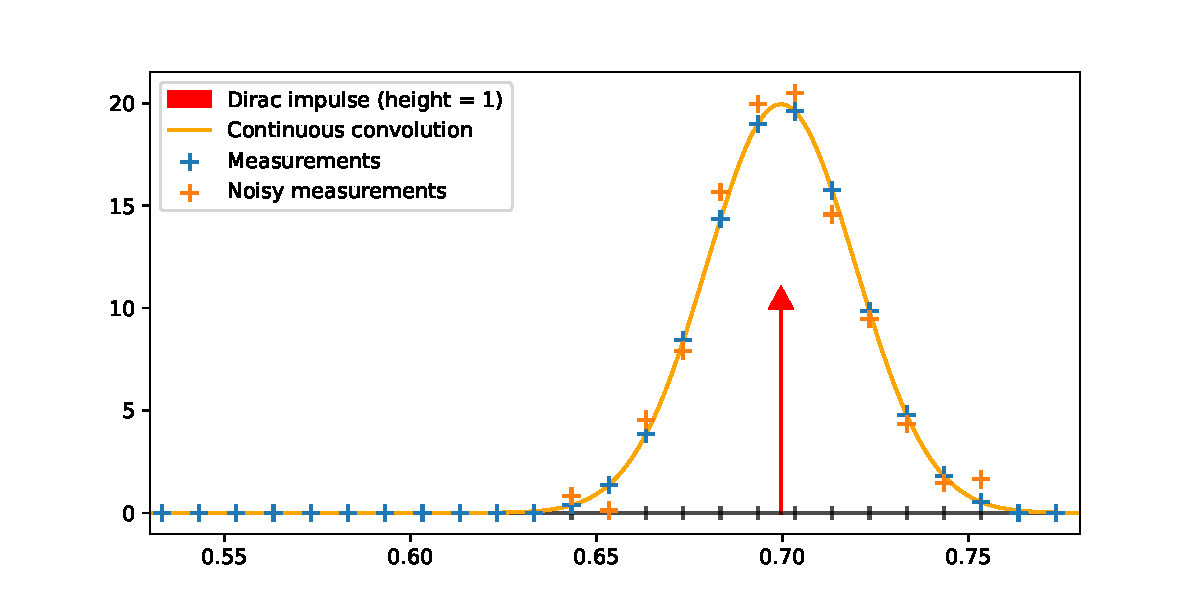
\includegraphics[width=\linewidth]{figures/simple_reco/measurement_figure.pdf}        
                \caption{Illustration of the effect of the measurement operator $\phib$ applied to a Dirac signal $\fb^\dagger = \delta_{x_0}$ with $x_0 \approx 0.695$.}
                \label{fig:simple:measop}
            \end{figure}

    
    \subsection{Composite representer theorem}

        As proposed, we address the deconvolution and signal separation task from \eqref{eq:ip-bis} using the two-variables optimization problem \eqref{eq:argminisback}. For a pair of parameters $\lambda_1, \lambda_2 > 0$ we consider

        \begin{equation}
        \label{eq:argmin-sps}
            \underset{(\fb,\fh) \in \mx \times \cHk}{\arg\min} \frac{1}{2} \| \bm{y} - (\phib (\fb) + \phih (\fh)) \|_2^2  + \lb \| \fb \|_{\mathcal{M}} + \frac{\lh}{2} \| \fh \|_{\cHk}^2.
        \end{equation}

        The solutions are indeed decoupled, according to the following result.
        \begin{proposition}
            \label{prop:rt-applied}
            Any solution to the optimization problem~\eqref{eq:argmin-sps} can be expressed as a pair of components $(s_1^*, s_2^*) \in \mx \times \cHk$ such that
            \begin{align}
                s_1^* &= \sum_{k=1}^{K_0} a_k \delta_{z_k}, \label{eq:deconv-banachpart}\\
                s_2^* &=  \frac{1}{\lh}\phih^* \mathbf{M}_{\lh}^{-1} \left(\bm{y} - \bm{w}\right),\label{eq:deconv-hilbertpart}
            \end{align}
            in which $(a_k, z_k)_k \in \left(\R \times \mathcal{X}\right)^{K_0} $ are amplitude-location pairs, $K_0 \leq L$, $\bm{w} = \phib(s_1^*)$ is independent on the actual solution $s_1^*$, and the matrix $\mathbf{M}_{\lambda_2} \in \R^{L \times L}$ is defined in equation \eqref{eq:def-Mphi}.
        \end{proposition}

        \begin{proof}
            By construction, Theorem~\ref{theo:main} holds for problem \eqref{eq:argmin-sps}. It directly leads to the expression of $s_2^*$ in $\eqref{eq:deconv-hilbertpart}$. Regarding the sparse component, we have that
            \begin{equation*}
                s_1^* \in \underset{ s_1\in\mx}{\arg\min} \quad  \mathcal{J}_{\mathbf{M}}(s_1)
            \end{equation*}
            with $\mathcal{J}_{\mathbf{M}}(s_1) := \|\mathbf{M}_{\lh}^{-\frac{1}{2}} ( \bm{y} - \phib(s_1)  ) \|_2^2  + \lb \| s_1 \|_{\mathcal{M}}$. From Proposition~\ref{prop:banachRT}, we know that this latter problem admits sparse solutions and that some can be expressed according to \eqref{eq:deconv-banachpart}.
        \end{proof}

        % \ju{Je mettrais le RT dans ce cas comme une proposition en étant clair sur le fait que c'est une application directe (à peine besoin d'une preuve)}
        % By construction, Theorem~\ref{theo:main} holds and the solution components are indeed decoupled.
        % With the matrix $\mathbf{M}_{\lambda_2} \in \R^{L \times L}$ defined in equation \eqref{eq:def-Mphi}, a solution of \eqref{eq:argmin-sps} is a pair of components $(s_1^\dagger, s_2^\dagger) \in \mx \times \ldx$ such that
        % \begin{align}
        %     s_1^* &\in \underset{ s_1\in\mx}{\arg\min} \quad  \mathcal{J}_{\mathbf{M}}(s_1), \label{eq:deconv-banachpart}\\
        %     s_2^* &=  \frac{1}{\lh}\phih^* \mathbf{M}_{\lh}^{-1} \left(\bm{y} - \bm{w}\right).\label{eq:deconv-hilbertpart}
        % \end{align}
        % with $\mathcal{J}_{\mathbf{M}}(s_1) = \|\mathbf{M}_{\lh}^{-\frac{1}{2}} ( \bm{y} - \phib(s_1)  ) \|_2^2  + \lb \| s_1 \|_{\mathcal{M}}$.
        % As stated in Theorem~\ref{theo:main}, $\bm{w} = \phib(s_1^*)$ does not depend on the recovered solution of \eqref{eq:deconv-banachpart}.
        % The smooth background problem \eqref{eq:deconv-hilbertpart} is explicit and only the sparse foreground estimation problem \eqref{eq:deconv-banachpart} needs to be solved numerically with optimization.
    
        % From Proposition~\ref{prop:banachRT}, we know that this latter problem admits sparse solutions and that some can be expressed as
        % \begin{equation*}
        %     s_1^* = \sum_k a_k \delta_{z_k}.
        % \end{equation*}
        
        The smooth background problem \eqref{eq:deconv-hilbertpart} is explicit, so that the only numerical challenge consists in estimating the positions $z_k \in \mathcal{X}$ and the associated intensities $a_k \in \R$ of the foreground component in \eqref{eq:deconv-banachpart}. The positions are notably more challenging to estimate than the intensities due to their continuously-defined nature and the nonlinear dependence on the measurements. This is done numerically by optimizing the single-component functional $\mathcal{J}_{\mathbf{M}}(\cdot)$ over $\mx$.
        The unique solution background component $s_2^*$ is then synthesized after computation of the residuals $\bm{y}-\bm{w}$ using \eqref{eq:deconv-hilbertpart}.

        \ad{
        \begin{remark}[Choice of the Hilbert space]
            The choice of the Hilbert space $\cH$ and in particular the Hilbert norm $\norm{\cdot}_\cH$ has a significant impact on the shape of $\fh^*$, involving the operator $\phih^*$ in equation~\eqref{eq:deconv-hilbertpart}. Classical choices consist in using the space of square integrable functions $\cH = \ldx$ equipped with the canonical norm $\norm{f}_{\ldx}^2 = \int_\cX f(x)^2 \mathrm{d}x$ for $f \in \ldx$, or alternatively introducing an invertible operator $\mathrm{L}_{\cH}: \ldx \to \ldx$ such that $\norm{f}_\cH^2 = \int_\cX \mathrm{L}_{\cH}\{f\}(x)^2 \mathrm{d}x $. However, these common norms generally do not permit to enforce a strong penalty on the high-frequency band of the solution, limiting their practical interest in applications.
            Our choice of using the RKHS induced by a Gaussian kernel is motivated by the test application considered in the following Section~\ref{sec:comp:reco}, in which we want to promote more energy in the low-frequency band. As demonstrated in equation~\ref{eq:rkhs-atom}, the reconstruction elements are shifted versions of the Gaussian function $g_t$ whose spatial extension is indeed larger than the measurement kernel $g$, hence promoting smoother solutions than what is achievable with classical $\mathrm{L}^2$-based norms.
        \end{remark}
        }
        
        % Finding a solution to \eqref{eq:deconv-banachpart} can then be reduced to the task of estimating some positions $z_k \in \mathcal{X}$ and the associated intensities $a_k \in \R$. The positions are notably more challenging to estimate than the intensities due to their their continuously-defined nature and the nonlinear dependence on the measurements.
        % The unique solution background component $s_2^*$ is then synthesized after computation of the residuals $\bm{y}-\bm{w}$ using \eqref{eq:deconv-hilbertpart}. 
        
    \subsection{Composite reconstruction}
    \label{sec:comp:reco}

        Some algorithms solve Problem \eqref{eq:argmin-sps}  directly on the continuum, such as the Sliding Frank-Wolfe \cite{denoyelle2019sliding} or the iterative refinement procedure of \cite{flinth2023grid}, however these methods can be long and computationally expensive to run.
        To put the emphasis on the decoupling of a composite solution, we decide here to simplify the solving by discretizing the foreground component estimation problem~\eqref{eq:deconv-banachpart}.
        
        % \ju{Question: ces méthodes peuvent résoudre un problem sparse comme (30) mais peuvent-elles résoudrent (29) en composite ?}\ad{Oui, si on utilise le RT de Debarre, qui permet de réduire la recherche de composante smooth en un problème de dimension finie. Dans ce cas, on peut calculer le gradient de (data fidelity + smooth regul) et appliquer les méthodes de types FW.}

    
        We do so by restricting the searched positions $z_k$ to live on a uniform fine grid. This approach alleviates the challenge of nonlinearity in the position parameters, turning \eqref{eq:deconv-banachpart} into a tractable finite dimensional generalized LASSO problem -- which can be large depending on the discretization interval and space dimensions. This strategy is usually adopted to approximate continuous-problem solutions \cite{simeoni2020functional,Debarre2019} and convergence toward gridless solutions has been studied (see \cite{duval2017sparseI,debarre2022part2} and the recent article \cite{guillemet2025a}). 
        % \ju{Tu peux ajouter le récent article de Vincent qui détaille cela plus loin que les autres résultats}

        We obtain the following finite-dimensional problem\footnotemark{} that approximates a continuous-domain solution of \eqref{eq:deconv-banachpart}:
        \begin{equation}
            \label{eq:gridbased-sparse}
            \underset{ \bm{a} \in \mathbb{R}^{J^d}}{\arg\min} \quad ( \bm{y} - \mathbf{H}\bm{a}  )^T \mathbf{M}_{\lh}^{-1} ( \bm{y} - \mathbf{H}\bm{a}  )  + \lb \| \bm{a} \|_{1},
        \end{equation}
        The $d$-dimensional grid contains $J^d$ knots and the vector $\bm{a}\in\R^{J^d}$ stores the amplitude of Dirac impulses located on the knots.
        The matrix $\mathbf{H} \in \R^{L \times J^d}$ accounts for the application of $\phib$ to grid-based Dirac impulses.
        In the simple case $d=1$, we obtain $\mathbf{H}[\ell, j] = g(x_{\ell} - z_j)$ for $1 \leq \ell \leq L $ and $1 \leq j \leq J$.
        \footnotetext{The discretization procedure is detailed in Appendix~\ref{app:discretization}.}
        
        The problem \eqref{eq:gridbased-sparse} can directly be solved with a proximal gradient descent algorithm (or any atomic LASSO solver such as a Frank-Wolfe algorithm). We solve this approximate problem considering a simple illustrative simulated example with $d=1$ in what follows.

        \subsubsection{Problem simulation and parametrization}

            We simulate a composite continuous-domain ground truth signal whose components are given by 
            $$s_1^{(0)} = \sum_{k=1}^{K_f} \beta_ k \delta(\cdot - u_k) \qquad\text{ and }\qquad s_2^{(0)} = \sum_{m=1}^{K_b} \gamma_m g_b(\cdot - v_m).
            $$
            The background component is built out of weighted replicas of the background Gaussian kernel $g_b = (1/\sqrt{2\pi\sigma_b^2}) \exp{(-x^2/(2 \sigma_b^2))}$ while the foreground involves sparse point sources. The locations $(u_k)_{k=1, \dots, K_f}$ and $(v_m)_{m=1, \dots, K_f}$ are drawn with a uniform distribution over the domain $[0, 1]$. The foreground is determined with $K_f = 10$ and $\beta_k$ drawn from a uniform distribution $\mathcal{U}([1, 10])$. The background parameters are $K_b = 100$ and $\gamma_m \sim \mathcal{U}([0.5, 1.5])$ with $\sigma_b = 0.08$.
            
            The measurement operator $\phib$ is defined with $L=100$ and $\sigma=0.02$. In addition, $\sigma_{\bm{n}}$ is set such that the signal-to-noise ratio between $\bm{y}$ and $\bm{n}$ reaches $SNR_\mathrm{dB} = 10 \log_{10}\left({\lVert \bm{y} \rVert_2^2}/{\lVert \bm{n} \rVert_2^2}\right) = 10$dB. To measure and adjust the contrast between the foreground and the background components in the signal to recover, we introduce the ratio $r_{1/2}$ of the contribution of each component in the observations, defined as
            \begin{equation}
                r_{1/2} = \frac{\lVert \phib (\fb^\dagger) \rVert_2 }{\lVert \phih (\fh^\dagger) \rVert_2 }.
            \end{equation}
    
            The observations $\bm{y}$ can be simulated with exact precision using this model. Indeed, we have
            $$
            \left[\phib(s_1^{(0)}) + \phih(s_2^{(0)})\right]_\ell = \sum_{k=1}^{K_f} \beta_k g(x_\ell - u_k) + \sum_{m=1}^{K_b} \gamma_m (g * g_b)(x_\ell - v_m),
            $$
            in which measuring the background involves the closed-form convolution
            $$
            (g\ *\ g_b)(x) = \frac{1}{\sqrt{2 \pi(\sigma^2 + \sigma_b^2)}} \exp{\left(-\frac{x^2}{2 (\sigma^2 + \sigma_b^2)}\right)}.
            $$
            
            We provide in figure~\ref{fig:simple:source} a simulated source signal built with a ratio of $r_{1/2} = 1$. 
            % \ju{après réflexion je me dis que tu peux garder la figure en expliquant bien l'effet d'échelle et le fait que la représentation peut être misleading.}
            The associated measurements are presented in figure~\ref{fig:simple:measurements}. Note that the contributions of the two components $\phib(\fb^\dagger)$ and $\phih(\fh^\dagger)$ have the same Euclidian norm although their distribution of mass is very different, leading to the misleading difference of scales in the right panel of figure~\ref{fig:simple:measurements}. %In this case, the $\ell_1$-norm of the contribution of the background is actually twice as large as the one from the foreground.
    
            \begin{figure}[t]
                \centering
                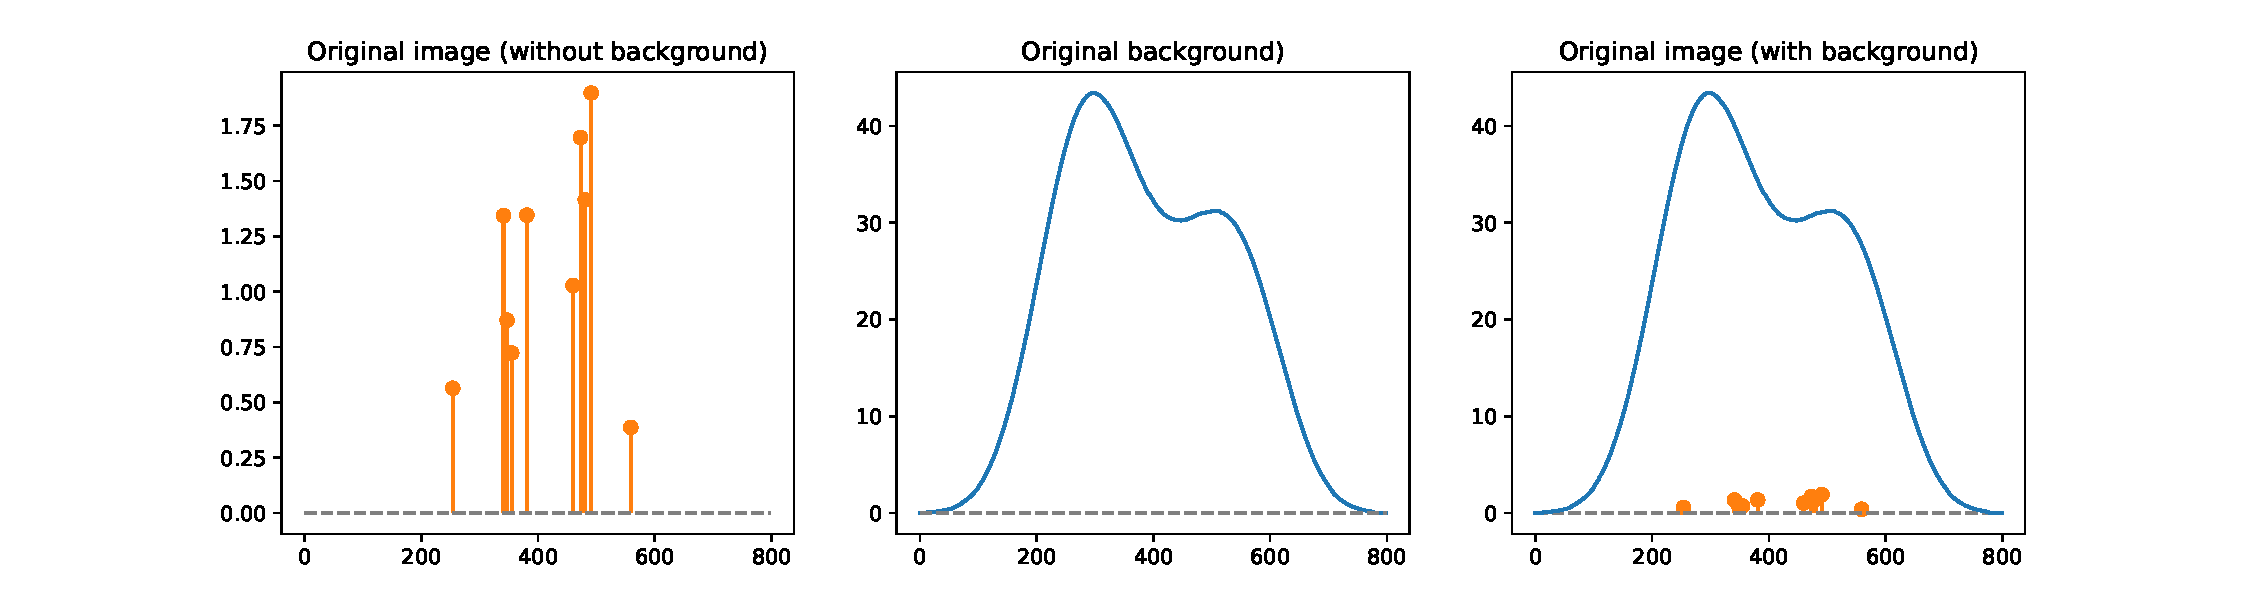
\includegraphics[width=\linewidth]{figures/simple_reco/gt.pdf}        
                \caption{Simulated source signal. \textit{Left:} Sparse component. \textit{Center:} Background smooth component. \textit{Right:} Sum of the two components.}
                \label{fig:simple:source}
            \end{figure}
        
            \begin{figure}[t]
                \centering
                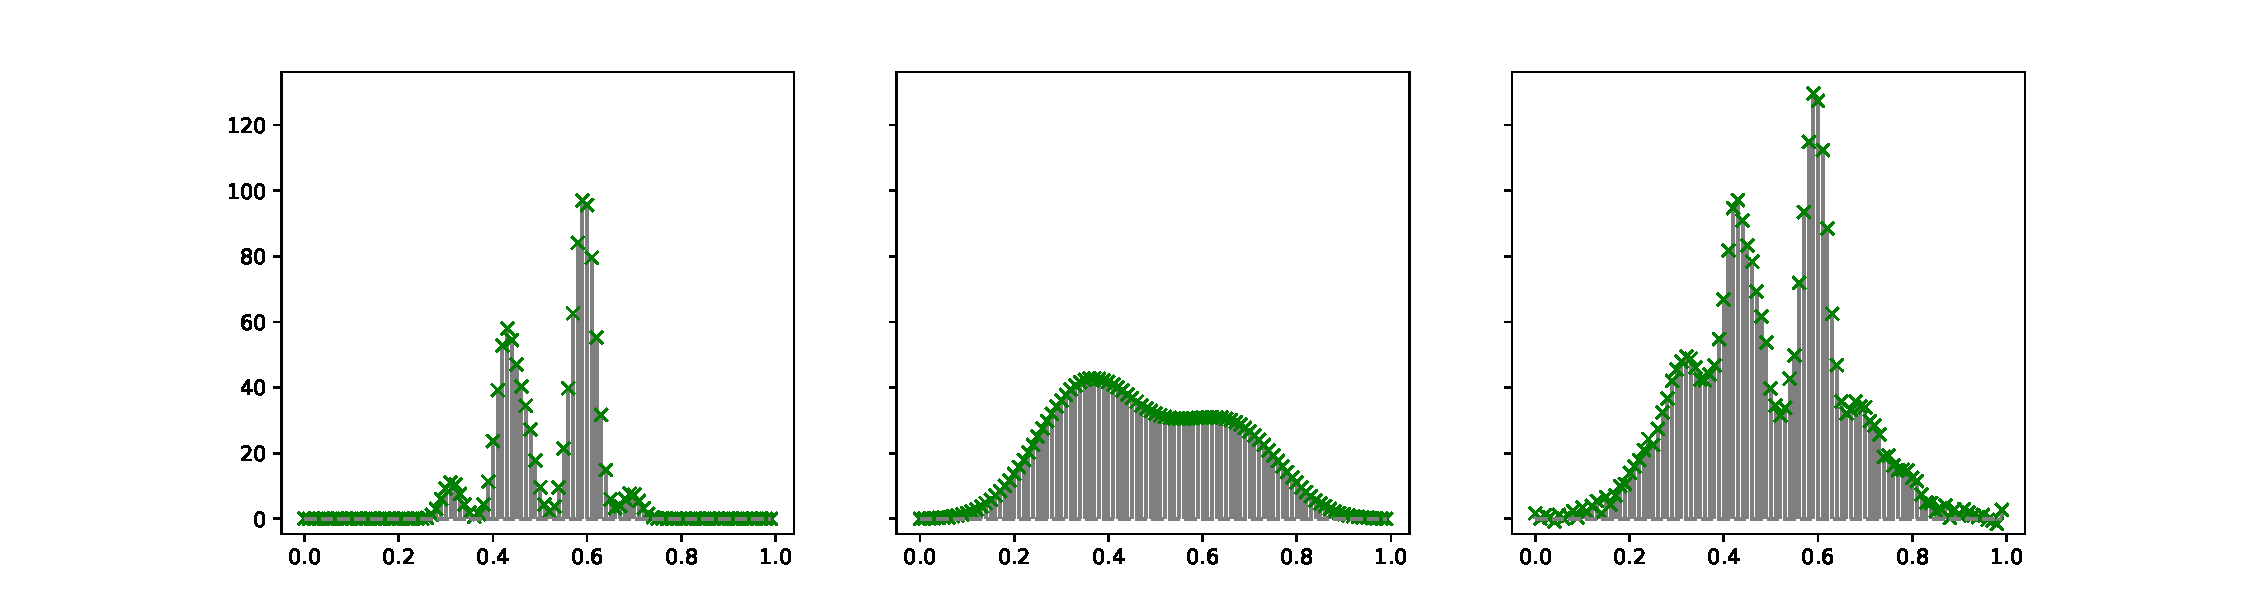
\includegraphics[width=\linewidth]{figures/simple_reco/measurements.pdf}        
                \caption{Simulated measurements. \textit{Left:} Contribution of the sparse component. \textit{Center:} Contribution of background. \textit{Right:} Total noisy observations $\bm{y}$. In practice, only the information of the right-hand plot are accessible and the problem does not know the respective contribution of the components.}
                \label{fig:simple:measurements}
            \end{figure}

        \subsubsection{Reconstruction of the signals}
        For a fine resolution reconstruction, the grid size is set to $J = n_\mathrm{srf} . L$ with the super-resolution factor fixed to $n_\mathrm{srf}=8$. The penalty parameters are tuned manually based on scaling rules to maintain values in a range consistent with the inverse problem. We set $\lh = \alpha_2 L$ with a real-valued coefficient $\alpha_2 >0$ (see Appendix~\ref{app:calculation} for a justification).
        %According to equation~\eqref{eq:def-Mphi}, the parameters $\lh$ appears in the sparse component estimation problem in front of the Gram matrix as $(1/\lh)\phih\phih^*$. It is then relevant to scale $\lh$ with the highest singular value of $\phih$, which is $\sigma_{mas}(\phih)\approx L$ in our case.
        Once $\lh$ has been set, $\lb$ is fixed as a rate of the maximum value as defined in \eqref{eq:l1max} with $\lb = \alpha_1 \lambda_{1, \mathrm{max}}$ for $0 < \alpha_1 <1$. Typically, $\alpha_1$ takes values in the range $[0.1, 0.3]$. To emphasize the smoothing effect on the background, we use the reconstruction width $\sigma_t = 0.1 > \sigma_b$.

        Figure~\ref{fig:simple:recos} presents the foreground and background components recovered with regularization parameters $\lambda_2 = 0.08 L =8$ and $\alpha_1 = 0.25$. Additionally, a positivity constraint has been enforced on $s_1$ which does not break the representer theorem and usually improves the quality of the reconstruction. We used an APGD algorithm \cite{liang2022improving} to solve the approximate decoupled problem \eqref{eq:gridbased-sparse}.

        \begin{figure}[t]
            \centering
            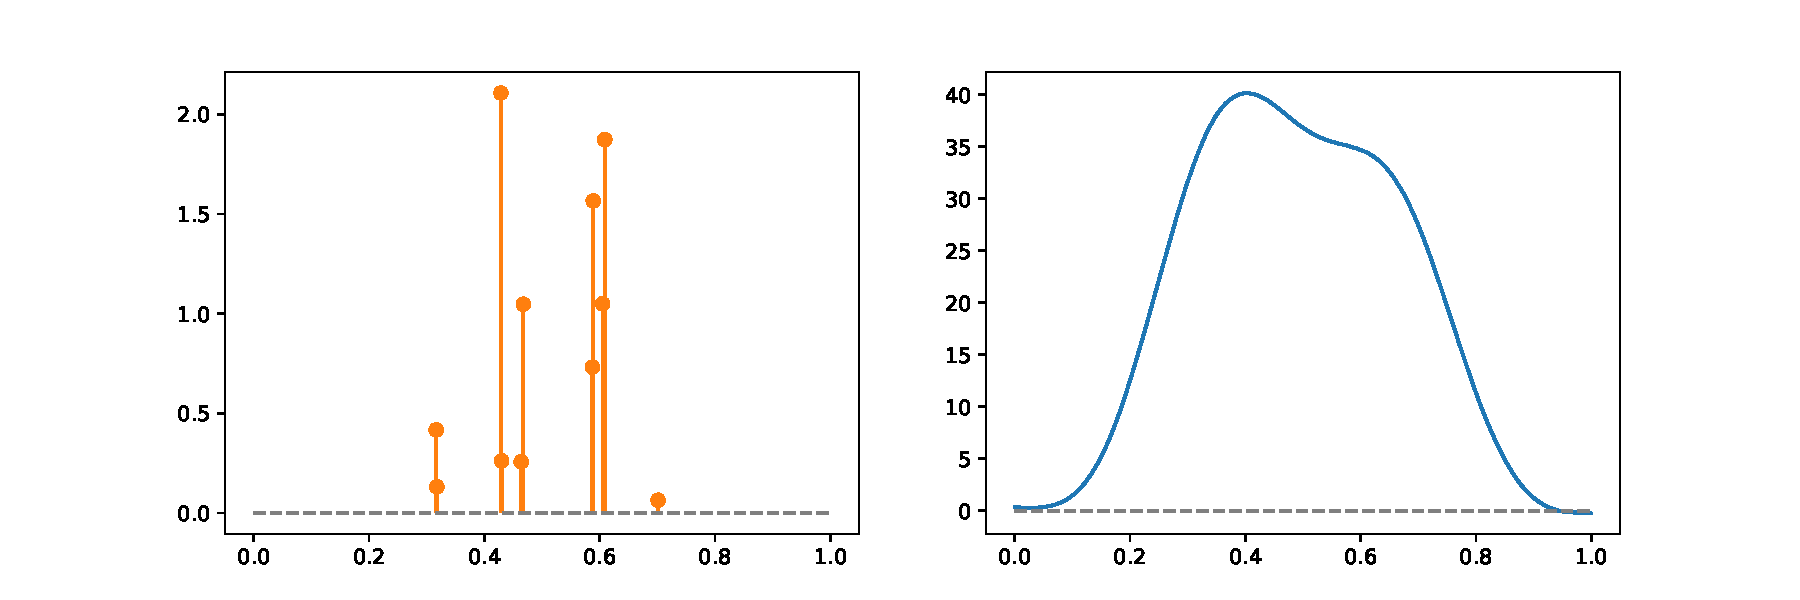
\includegraphics[width=\linewidth]{figures/simple_reco/recos.pdf}        
            \caption{Recovered signals with regularization parameters $\lambda_2 = 10^{-2}$ and $\alpha = 0.2$. \textit{Left:} Sparse foreground component. \textit{Right:} Smooth background.}
            \label{fig:simple:recos}
        \end{figure}

        The sparse component is similar to the simulated source signal of figure~\ref{fig:simple:source} although many reconstructed peaks are composed of several small intensity impulses, which makes the comparison with the ground truth difficult. The background component is less faithful. The overall intensity matches the intensity of the ground truth but the local variations are not correctly captured, we observe for instance high intensity around the coordinate $0.7$ which could correspond to a leakage from the foreground component. Additionally, we  observe a plateau effect in the recovered background information, reaching here the value $35$. This plateau is systematic in the reconstructions (as can be seen in Appendix~\ref{app:reconstructions}) and could be due to the LASSO problem, which outputs a residual of bounded intensity.

        This difficulty to accurately recover the background may not be critical in practice as one is usually interested in accurate reconstruction of the foreground component. To provide a better comparison between the source foreground component and the recovered one, we convolve the sparse signals $s_1^*$ and $s_1^\dagger$ with a representation kernel. We use a narrow Gaussian function of small standard deviation $\sigma_r = \sigma/4$. This operation intuitively blends nearby peaks while respecting the spatial spread of different clusters. The resulting signals are displayed in figure~\ref{fig:simple:recos-conv}, demonstrating consistency between the signals.
        % \ad{Should I comment more ?}
        % The $K_f=10$ source peaks are recovered. Some of them suffer from a small intensity shrinkage, which is a well-known artefact of LASSO-like problems. Spurious peaks are also reproduced around the left peak, which may be explained by the presence of strong background information around this location. 
        
        \begin{figure}[t]
            \centering
            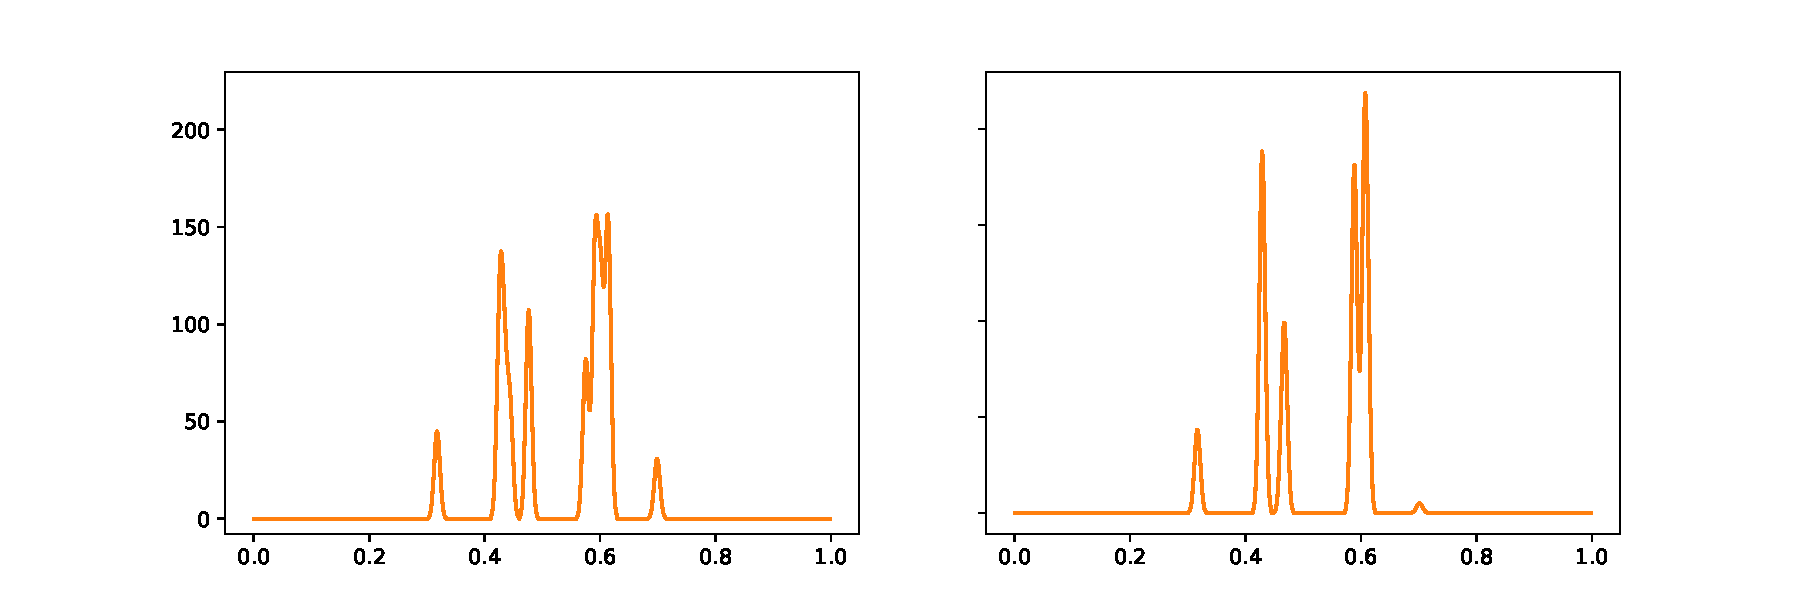
\includegraphics[width=\linewidth]{figures/simple_reco/recos_conv.pdf}        
            \caption{Foregrounds convolved with the sharp representation kernel. \textit{Left:} Ground truth signal. \textit{Right:} Reconstruction.}
            \label{fig:simple:recos-conv}
        \end{figure}

        Obviously, the penalty parameters $\lb$ and $\lh$ have a significant influence on the recovered components and the interplay between the respective value of these two parameters is not fully understood. We provide in Appendix~\ref{app:reconstructions} a cross table of reconstructions with various regularization parameters to illustrate the dependence. 
        
\section{Benefits of our Decoupled Composite Model}
    
    Building on the simulated composite model presented in the previous section, we now illustrate the benefits of our approach.
    
    First, composite modeling accurately recovers the unknown signal in situations where single-component problems fail to distinguish foreground from background information. Second, using a decoupled numerical procedure reduces the computation time compared to a direct 2-variables approach of the composite optimization problem.

    The numerical experiments in this section have been implemented with the Python programming language based on the optimization package \texttt{Pyxu} \cite{pyxu-framework}. All the simulations have run on a workstation with 2 CPUs Intel Xeon E5-2680 v3 \@2.5 Ghz, 30 MB cache and 24 threads each. 

    \subsection{Compared to single-component model}
    \label{sec:bene:comp}
        In applications where only the foreground component is of interest, we may wonder if using a composite model is relevant in the first place. Would it be possible to simply recover the foreground with a single-component sparsity-promoting problem only? We address the question in this section, first visually then introducing evaluation metrics.

        \subsubsection{Single-component reconstruction}
        Using the same composite ground truth signal $(s_1^\dagger, s_2^\dagger)$ as in Section~\ref{sec:comp:reco}, we consider the following single-component B-LASSO problem with still the same measurement operator $\phih$ and the same observations $\bm{y}\in\R^L$:
        \begin{equation}
            \label{eq:argmin-sparse-only}
            \underset{\fb \in \mx}{\arg\min} \frac{1}{2} \| \bm{y} - \phib (\fb) \|_2^2  + \lambda \| \fb \|_{\mathcal{M}},
        \end{equation}
        for $\lambda > 0$.
        With the fine-grid discretization proposed above, finding an approximate grid-based solution of this problem amounts to solve a classical LASSO problem. The regularization parameter $\lambda > 0$ is set specifically for this problem and is independent of $\lb$ used in \eqref{eq:deconv-banachpart}. There also exists a maximum value $\lambda_\mathrm{max} = \norm{\phib^*\bm{y}}_\infty$ for problem~\eqref{eq:argmin-sparse-only} and we set $\lambda = \alpha \lambda_\mathrm{max}$ for $0 < \alpha < 1$. It is usually larger than $\lambda_1$ as we need stronger prior information to recover a sparse solution.
        
        Figure~\ref{fig:simple:blasso-conv} displays the reconstructions with the same representation kernel as before for various reconstruction parameters $\alpha$.
        We observe that the B-LASSO problem manages to recover some high intensity peaks, however the reconstructions are strongly corrupted by the presence of background information. When more sparsity is enforced with a larger value of $\alpha$, the spurious peaks tend to vanish but the intensity of the relevant peaks is also reduced, becoming lower than the source and than the composite reconstruction.

        \begin{figure}[t]
            \centering
            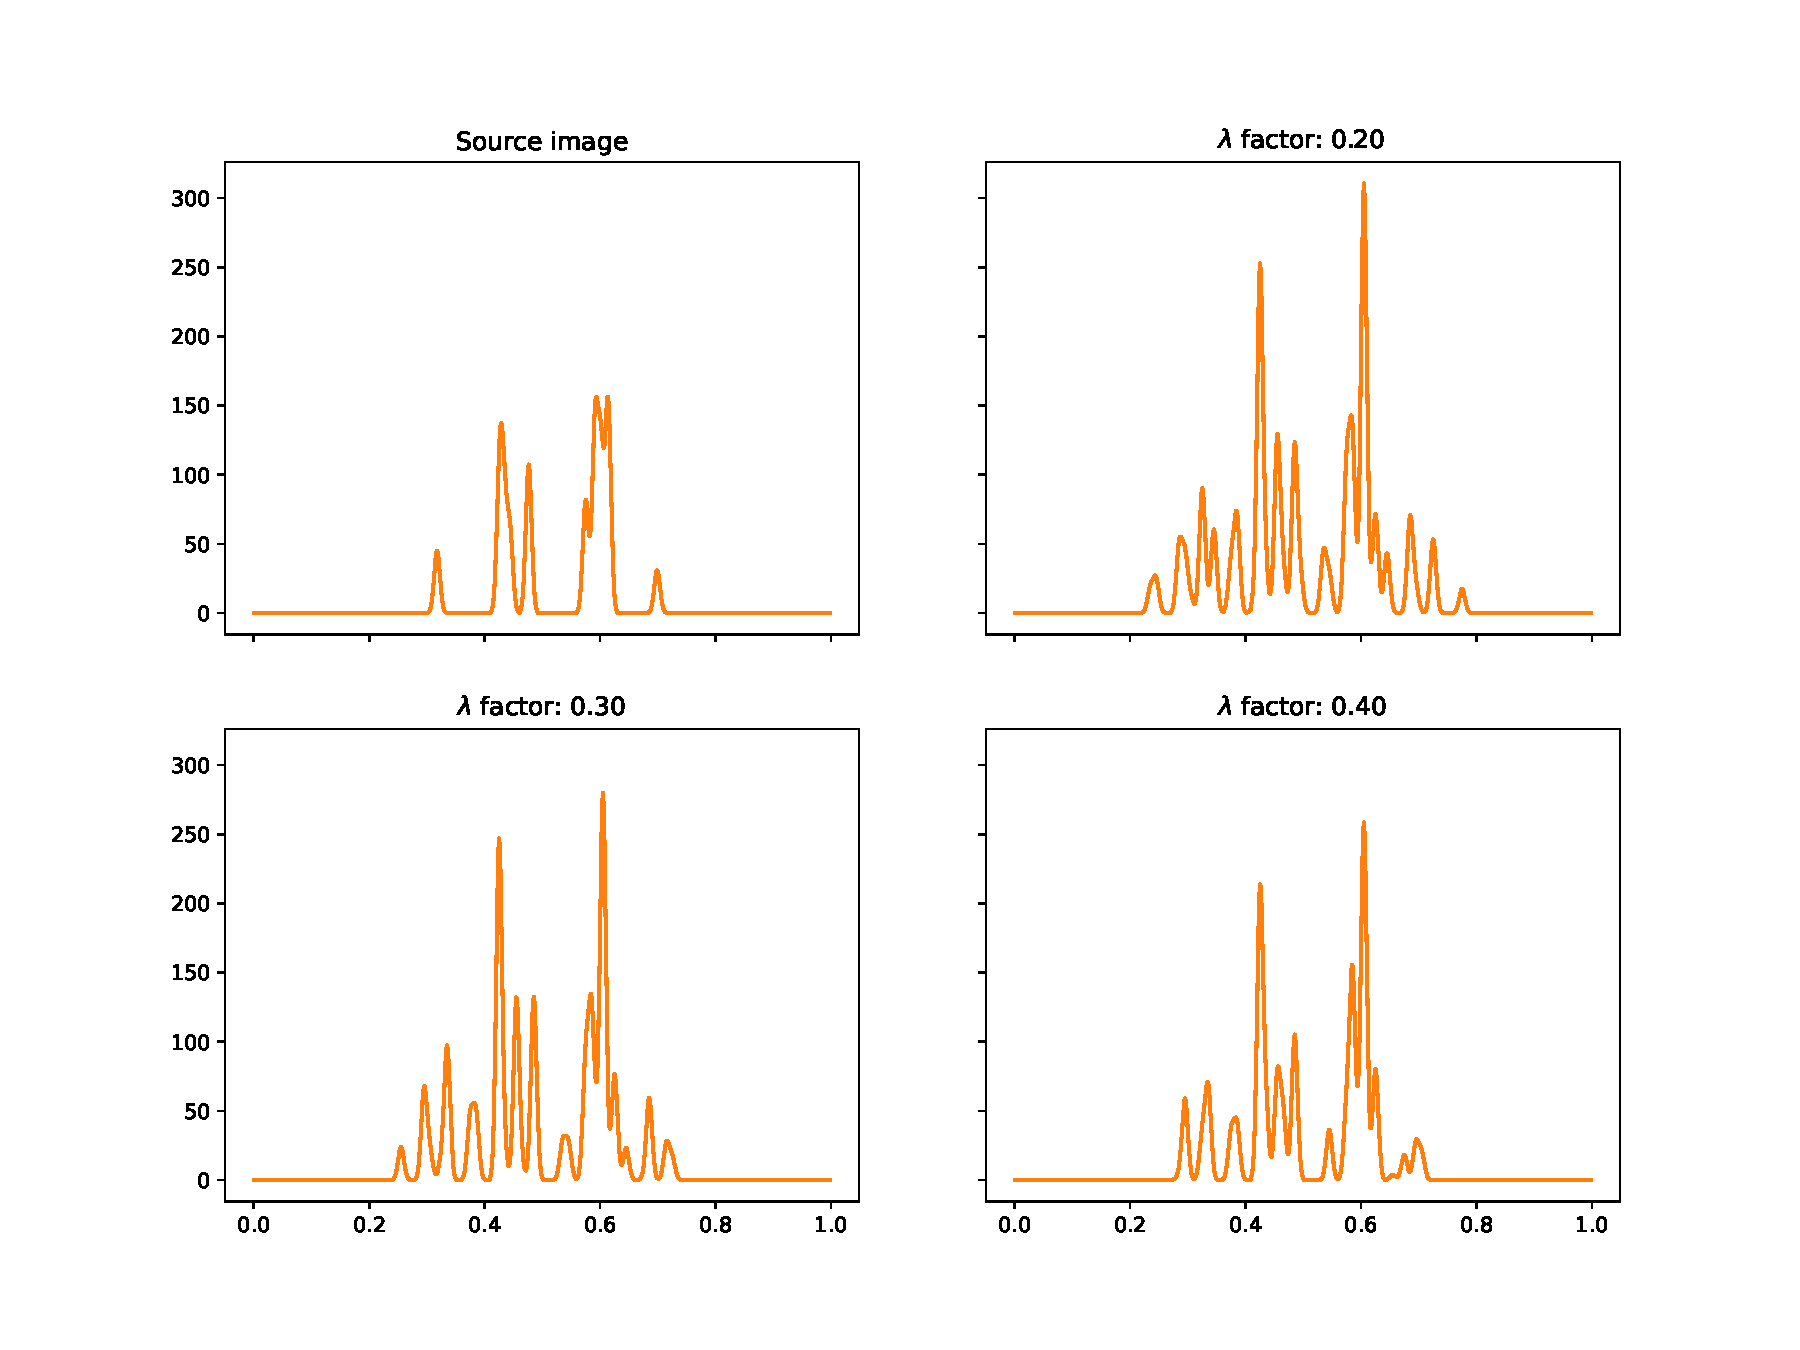
\includegraphics[width=\linewidth, trim=0 2cm 0 2.2cm, clip]{figures/simple_reco/blasso_merged.pdf}
            \caption{Single-component reconstructions using a B-LASSO problem approximated on the fine grid: ground truth (\textit{upper left}) and several values of the regularization parameter ($\alpha=0.2, 0.3$ or $0.4$). \ad{Larger titles or subfigures.}}
            \label{fig:simple:blasso-conv}
        \end{figure}
        
        \subsubsection{Quantitative study}

        Assessing the quality of the reconstruction of sparse signal is always a complicated task as both intensity and localization of the recovered sources need to be simultaneously evaluated. We consider two simple metrics based on the grid-based representation of the recovered foreground. First, the ground truth and the solution are convolved with the representation Gaussian kernel. Second, the relative error is computed using either $\mathrm{L}^2$-norm or the $\mathrm{L}^1$-norm. For $\fb$ the recovered foreground component, $\fb^\dagger$ the simulated source and $g_{\sigma_r}$ the representation kernel, we define
        $$
        \mathrm{RE}_2(\fb, \fb^\dagger) = \frac{\lVert g_{\sigma_r} * (\fb - \fb^\dagger) \rVert_2 }{ \lVert g_{\sigma_r} * \fb^\dagger \rVert_2} \qquad\text{and}\qquad
        \mathrm{RE}_1(\fb, \fb^\dagger) = \frac{\lVert g_{\sigma_r} * (\fb - \fb^\dagger) \rVert_1}{\lVert g_{\sigma_r} *\fb^\dagger \rVert_1}.
        $$
        The metrics are approximated using the fine-grid representation of the signals.

        The evaluation metrics on the foreground component are reported in tables~\ref{tab:rl2} and~\ref{tab:rl1} for the sparse-plus-smooth composite model, and in table~\ref{tab:blasso} for the single-component reconstructions with the B-LASSO. The parameters chosen for figures~\ref{fig:simple:recos} and~\ref{fig:simple:recos-conv} correspond to the best pair $\lambda_2 = 0.08 L$ and $\alpha_1=0.25$, the reconstructions obtained with the other parameters are displayed in Appendix~\ref{app:reconstructions}.

        % The best B-LASSO reconstruction is consistently outperformed by most of the composite reconstructions. \ju{Comme dit ailleurs, je ne comprends pas pourquoi les expériences te permettent de dire ça vu que tu considère deux problèmes différents. Pourquoi ne pas prendre $s$ au lieu de $s_1$ qui montrerait que le Lasso a visuellement et quantitativement mieux ? To be discussed.}
        The two metrics produce consistent results as they both identify the same best solution, although the values and the gaps between the methods are different. The metrics for the B-LASSO improve with higher values of the penalty parameter, coincidentally with a decrease in intensity of the recovered signal. This observation may suggest that the B-LASSO model is inappropriate for such a recovery problem and having a composite model improves the reconstruction. 
        
        \begin{table}[b]
        \centering
        \begin{subtable}[t]{0.45\linewidth}
            \centering
            \begin{tabular}{l|rrrr}
                \toprule
                 & \multicolumn{4}{c}{$\alpha_2$ in $\lambda_2 = \alpha_2 L$} \\
                \cmidrule(lr){2-5}
                $\alpha_1$ & 0.80 & 4.00 & 8.00 & 40.00 \\
                \midrule
                0.02 & 0.503 & 0.728 & 0.798 & 1.047 \\
                0.05 & 0.567 & 0.592 & \textbf{0.440} & 1.075 \\
                0.10 & 0.637 & 0.595 & 0.571 & 0.839 \\
                0.15 & 0.826 & 0.805 & 0.647 & 0.516 \\
                \bottomrule
            \end{tabular}
            \caption{Relative $\ell_2$-norm error \label{tab:rl2}}
        \end{subtable}
        \hfill
        \begin{subtable}[t]{0.45\linewidth}
            \centering
            \begin{tabular}{l|rrrr}
                \toprule
                 & \multicolumn{4}{c}{$\alpha_2$ in $\lambda_2 = \alpha_2 L$} \\
                \cmidrule(lr){2-5}
                $\alpha_1$ & 0.80 & 4.00 & 8.00 & 40.00 \\
                \midrule
                0.02 & 0.495 & 1.070 & 1.297 & 1.748 \\
                0.05 & 0.585 & 0.601 & 0.626 & 1.669 \\
                0.10 & 0.647 & 0.593 & \textbf{0.571} & 1.196 \\
                0.15 & 0.802 & 0.790 & 0.661 & 0.600 \\
                \bottomrule
            \end{tabular}
            \caption{Relative $\ell_1$-norm error\label{tab:rl1}}
        \end{subtable}
        \caption{Evaluation metrics for the composite reconstructions.}
        \end{table}
    
        \begin{table}[b]
            \centering
            \begin{tabular}{l|rrrr}
                \toprule
                 & \multicolumn{4}{c}{$\alpha$ in $\lambda = \alpha \lambda_{\mathrm{max}}$} \\
                \cmidrule(lr){2-5}
                 & 0.10 & 0.20 & 0.30 & 0.40 \\
                \midrule
                $\mathrm{RE}_2$ & 1.126 & 1.033 & 0.953 & \textbf{0.783} \\
                $\mathrm{RE}_1$ & 1.864 & 1.593 & 1.370 & \textbf{1.051} \\
                \bottomrule
            \end{tabular}
            \caption{B-LASSO errors \label{tab:blasso}}
        \end{table}

        To further compare the interest of using a composite model over a single-component one, we study how the reconstruction metrics evolve with respect to the contrast of the signal to recover, that is the relative importance between the foreground and background components. We run the same experiment while varying the parameter $r_{1/2}$ and we report in figure~\ref{fig:bench:metrics-vs-r} the best value of the metric obtained through various sets of regularization parameters.

        Independently of the contrast and the metric used, the composite model systematically outperforms the single-component one. With higher values of contrast, that is when the foreground gets more intense relative to the background, both model reduce their error metrics and thus produce better reconstructions. Interestingly, the gap between the methods also shrinks with the contrast, ultimately being almost nonexistent for $r_{1/2} = 4$. It suggests that for sufficiently high contrasts, sparse single-component modeling may be enough to obtain an accurate reconstruction of the foreground.

        \begin{figure}[t]
            \centering
            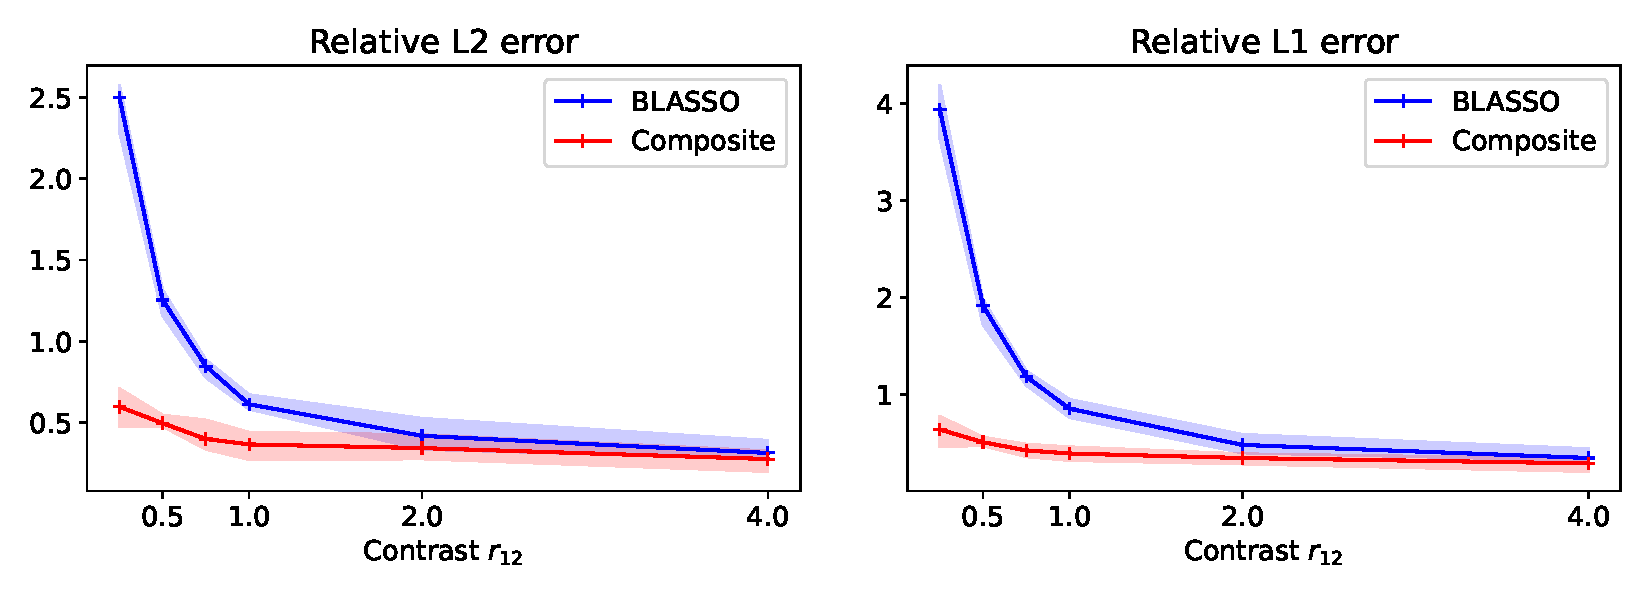
\includegraphics[width=\linewidth]{figures/benchmark/error_vs_r12.pdf}        
            \caption{Relative error with respect to contrast. For each value of $r_{1/2}$, 24 problems are simulated and solved, the median values and interquartile spreads are respectively shown with solid line and shaded area. \textit{Left:} Using $RE_2$. \textit{Right:} Using $RE_1$.}
            \label{fig:bench:metrics-vs-r}
        \end{figure}


    \subsection{Compared to a non-decoupled solver}
    \label{sec:bene:deco}
        So far we have illustrated Theorem~\ref{theo:main} and highlighted the interest of using a composite model in the presence of a smooth background signal. The main contribution of our theorem consists in the decoupling of the composite optimization problem and its practical benefits unveil when comparing the solving time with a direct non-decoupled approach. 

        \subsubsection{Non-decoupled approach}
        Letting apart Theorem~\ref{theo:main}, the composite optimization \eqref{eq:argmin-sps} can also be treated directly using the representer theorem of \cite{debarre2021continuous}. Indeed, it was known that there exists at least one Dirac-based sparse solution for the foreground component as
        \begin{equation}
            s_1^* = \sum_{k=1}^{K_1} a_{k} \delta(\cdot - x_k)
            \label{eq:rt-deb-1}
        \end{equation}
        with $a_{k} \in \mathbb{R}$, $x_k \in \mathcal{X}$ and $K_1 \leq L$.
        Additionally, the background component was known to be unique and that it can be expressed as
        \begin{equation}
            s_2^* = \sum_{\ell=1}^{L} b_{\ell} \phi_\ell,
            \label{eq:rt-deb-2}
        \end{equation}
        with $b_\ell \in \mathbb{R}$ and $\phi_\ell$ the measurement functionals.

        Plugging \eqref{eq:rt-deb-1} after discretization on the fine grid $G_J$ and \eqref{eq:rt-deb-2} into the composite minimization cost function \eqref{eq:argmin-sps}, we obtain the following two-components optimization problem of dimension $J^d + L$, that we refer to as the \emph{non-decoupled approach} :
        \begin{equation}
        \label{eq:ndcp-argmin}
            \underset{(\mathbf{a}, \mathbf{b})\ \in\ \R^{J^d} \times \R^L}{\arg\min} \frac{1}{2} \| \bm{y} - \mathbf{Ha} - \mathbf{Tb} \|_2^2  + \lb \| \mathbf{a} \|_1 + \frac{\lh}{2} \langle \mathbf{b}, \mathbf{Tb} \rangle,
        \end{equation}
        where the matrix $\mathbf{T} \in \R^{L \times L}$ is defined as
        % $\mathbf{T}[i, j] = \langle \phi_j, \phi_i\rangle$ for $1 \leq i, j \leq L$
        $\mathbf{T}[i, j] = (g * g_0 * g)(x_j - x_i)$ for $1 \leq i, j \leq L$
        and $\mathbf{H} \in \R^{L\times J^d}$ is from \eqref{eq:gridbased-sparse}.
        % \ju{do you specify what is $T$ and how it connects with our theorem? + recall what is $H$ maybe.}
        This problem is equivalent to our decoupled and discretized approach \eqref{eq:deconv-banachpart} and \eqref{eq:deconv-hilbertpart}. It is convex, finite-dimensional, and the terms are either differentiable or proximable so that the optimization can be performed with a proximal algorithm. In what follows, we solve it with APGD. % and refer to this approach as \emph{non-decoupled}.
    
        \subsubsection{Quantitative assessment}
        As mentioned with Proposition~\ref{prop:rt-applied}, the composite optimization problem \eqref{eq:argmin-sps} can be solved by performing an optimization procedure on the foreground component only.
        %The numerical procedure get simplified as only one variable needs to be considered.
        To asses the practical benefits of such transformation, we compare the runtime of the decoupled solver, including the a posteriori computation of the background component, with the non-decoupled approach of solving the two-components problem~\eqref{eq:ndcp-argmin}. For completeness, we also include in our comparison the runtime for solving a B-LASSO problem with the same input.

        For a fair treatment between the solver, the stopping criterion of all the algorithms is set as a threshold on the relative improvement of consecutive iterates of the foreground component variable. We present two experiment: the first one, displayed in figure~\ref{fig:time-vs-r}, reports the reconstruction time when the contrast $r_{1/2}$ evolves in the same setup as in section~\ref{sec:bene:comp}; the second experiment is reported in figure~\ref{fig:time-vs-srf} and presents the reconstruction time when the super resolution factor $n_\mathrm{srf}$ varies. The times reported correspond to the best reconstruction obtained through a tested set of regularization parameters. Each experiment is reproduced 24 times, the median value is reported with the solid line and the shaded area represents the interquartile spread.
        % \ju{I don't see where NDCP is presented, commented and linked with some previous works. I am right?}

        \begin{figure}[t]
            \centering
            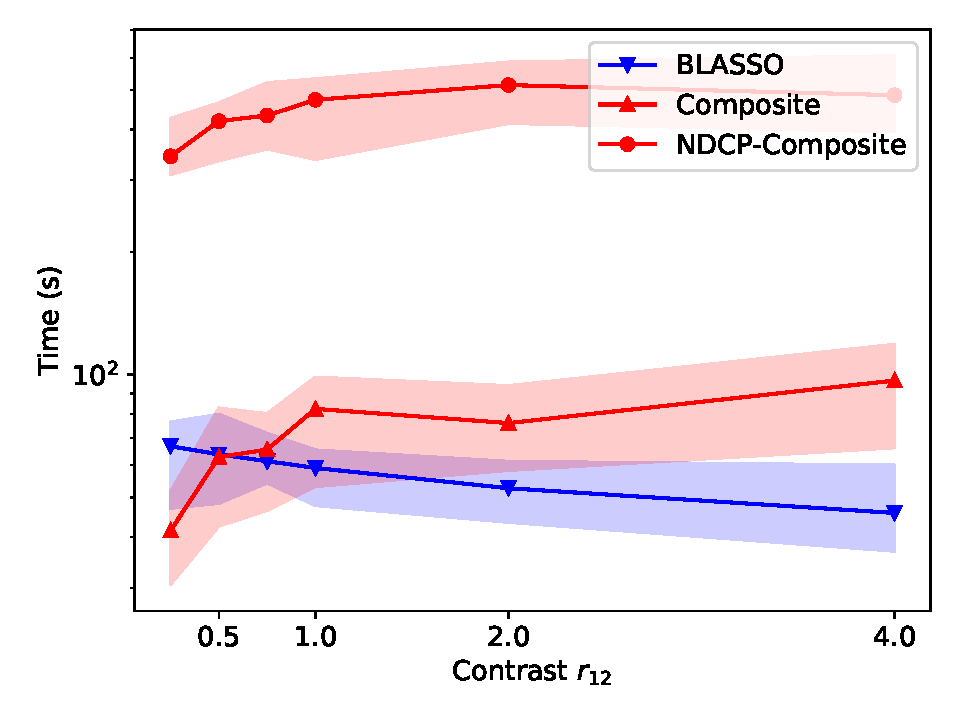
\includegraphics[width=.7\linewidth]{figures/benchmark/time_vs_r12.pdf}        
            \caption{Time for the best reconstruction with the different solvers with varying values of $r_{1/2}$ and fixed value of $n_\mathrm{srf} = 8$. The two composite approaches are in red, with triangle markers for the decoupled reconstruction and circle for the non-decoupled problem (``NDCP'' in the legend).}
            % \ju{I wonder what happens with a log scale. We shall see more easily the gain with the BLASSO.}
            \label{fig:time-vs-r}
        \end{figure}
    
        \begin{figure}[t]
            \centering
            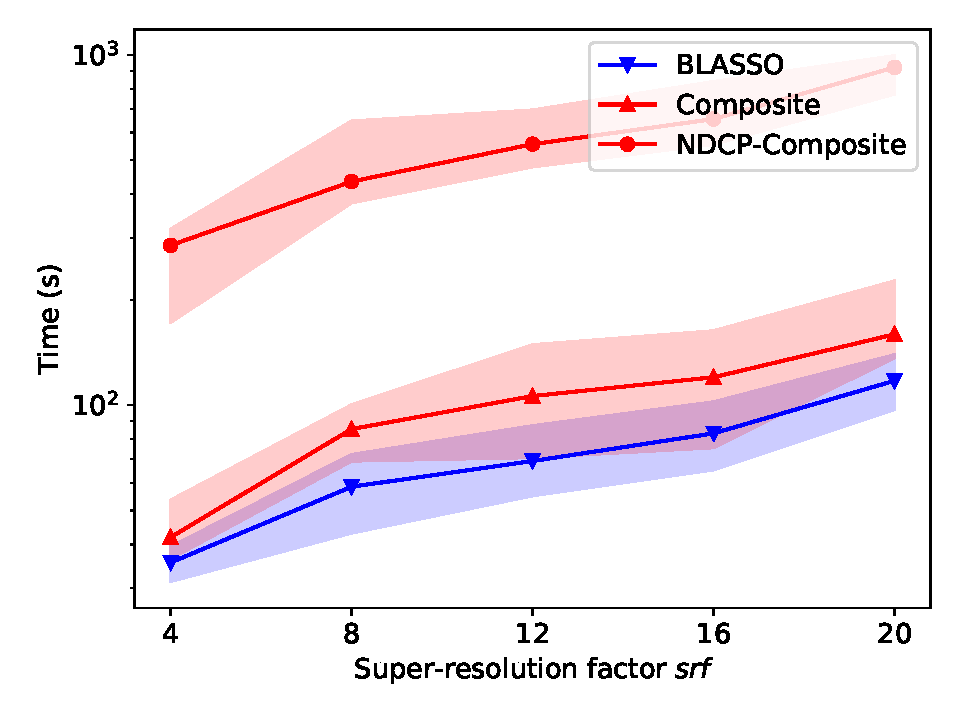
\includegraphics[width=.7\linewidth]{figures/benchmark/time_vs_srf.pdf}        
            \caption{Time for the best reconstruction with the different solvers with varying values of $n_\mathrm{srf}$ and fixed $r_{1/2}=1$.}
            \label{fig:time-vs-srf}
        \end{figure}
    
        \ad{Update the figures.}
        On both scenarios, the decoupled approach run significantly faster than the non-decoupled one, on average taking 10.6\% of the runtime in the first experiment (varying contrast) and 8.9\% in the second one (varying super resolution factor). Up to numerical approximations, the solutions are identical between the two methods. Interestingly, the decoupled approach turns out to be faster than the regular B-LASSO solver. Varying the contrast $r_{1/2}$ has little effect on the reconstruction time. Increasing the resolution, that is using more grid points in the discrete representation of $s_1^*$, slows down the solving for all the algorithms. The effect is stronger for the non-decoupled method, which suffers from having its reconstruction time multiplied by approximately $3.5$.

        

\section{Conclusion}

    % \begin{itemize}
    %     \item Composite approach for inverse problem
    %     \item Revisit the Sparse-plus-Smooth problem of Debarre et al.
    %     \item General decoupling result when the problems are simple
    %     \item Main benefit: decoupled numerical solver, much faster
    %     \item Illustration of the relevance of composite model (even in a simple case)
    %     \item Further work: Application to microscopy or astronomy.
    % \end{itemize}

    We introduced a new representer theorem for composite sparse-plus-smooth optimization problems, revisiting the original result from~\cite{debarre2021continuous}. Our theorem investigates deeper the connection between the two components of the problem and demonstrates a form of decoupling between them. Interestingly, the composite minimization can be transformed into an equivalent simpler single-component problem. We recover the uniqueness of the smooth component and provide a more precise closed-form expression depending on the residual of the decoupled sparse problem.

    We highlighted the relevance of composite models for sparse recovery when the observations are corrupted with the presence of background information, in scenarios where single-component sparse modeling only fails to produce accurate solutions. Moreover, the decoupled numerical procedure stemming from our representer theorem significantly outperforms the direct two-variable approach in terms of solving time.

    Building on this fast solver, composite models could be used as an enhanced version of traditional sparsity-promoting methods for practical applications involving large measurement datasets, such as 2D and 3D SMLM deconvolution.

    % \ad{Reference to lensless imaging as potential application ?}


% \ack 
\section*{Acknowledgments}
    The authors sincerely thank Martin Vetterli for his trust and guidance throughout this project.   
    A.J. is funded by the Swiss National Science Fundation (SNSF) under grant \emph{SESAM - Sensing and Sampling: Theory and Algorithms (n\textdegree 200021\_181978/1)}.
    
\clearpage
\appendix

\section{Proof of Theorem~\ref{theo:main}}
\label{app:prooftheo1}

    Let us recall the composite problem of interest. For $\lambda_1, \lambda_2 > 0$ we write the objective functional as
    \begin{equation*}
        \mathcal{J}(\fb, \fh) := \frac{1}{2} \| \bm{y} - (\phib (\fb) + \phih (\fh)) \|_2^2  + \lb \| \fb \|_{\mathcal{B}} + \frac{\lh}{2} \| \fh \|_{\mathcal{H}}^2.
    \end{equation*}
    
    % \begin{proof}
    
    % We define the cost function 
    % \begin{equation*}
    %     \mathcal{J}(\fb, \fh)
    %     =\| \bm{y} - (\phib (\fb) + \phih (\fh)) \|_2^2  + \lb \| \fb \|_{\mathcal{B}} + \lh \| \fh \|_{\mathcal{H}}^2.
    % \end{equation*}
    Assume first that $\fb$ is fixed and consider the optimization problem $\inf_{s_2 \in \mathcal{H}} \mathcal{J}(\fb, \fh)$. It is clearly equivalent to
    \begin{equation*}
        % \mathcal{U} ( (\bm{y} - \phib(\fb)), \phih, \lh) =
        \underset{\fh \in \mathcal{H}}{\arg\min}  \quad \frac{1}{2} \| (\bm{y} - \phib(\fb)) - \phih(\fh) \|_2^2 + \frac{\lh}{2} \| \fh \|_{\mathcal{H}}^2,
    \end{equation*}
    whose unique solution according to Proposition~\ref{prop:hilbertRT}, depends on $\fb$ and is given by
    \begin{equation}
        \label{eq:hatfwithfb}
        \widehat{s}_{2, \fb} =\phih^* ( \phih \phih^* + \lh \mathbf{I}_L)^{-1} ( \bm{y} - \phih(\fb) ). 
    \end{equation}
    Using the latter relation, we therefore deduce that $(\hfb,\hfh) \in \mathcal{W} (\lb,\lh)$ if and only if  
    \begin{align}
        \hfh &= \widehat{s}_{2,\hfb} = \phih^* ( \phih \phih^* + \lh \mathbf{I}_L)^{-1} ( \bm{y} - \phib(\hfb) ) , \quad \text{and} \label{eq:findmethishfh}\\
        \hfb &\in\underset{\fb \in \mathcal{B}}{\arg\min}  \quad \mathcal{J}(\fb, \widehat{s}_{2, \fb}) \label{eq:newhproblem}
    \end{align}
    % where
    % \begin{equation}
    % \label{eq:newcostfb}
    %     \mathcal{J}(\fb) = \| \bm{y} - \phih( \widehat{f}_{2, \fb} ) -  \phib (\fb) \|_2^2 + \lb \| \fb \|_{\mathcal{B}} + \lh \|  \widehat{f}_{2, \fb}\|_{\mathcal{H}}^2.
    % \end{equation}

    Replacing $\widehat{s}_{2, \fb}$ with its expression~\eqref{eq:hatfwithfb}, we observe that
    \begin{align}
        \| \bm{y} - \phih( \widehat{s}_{2, \fb} ) - \phib (\fb) \|_2^2 &= 
        \| (\mathbf{I}_L - \phih \phih^*( \phih \phih^* + \lh \mathbf{I}_L)^{-1}) ( \bm{y} - \phib (\fb) ) \|_2^2 \nonumber  \\
        &= \lh^2 \| ( \phih\phih^* + \lh \mathbf{I}_L)^{-1} (\bm{y} - \phib(\fb) ) \|_2^2 \label{eq:firstinterm}
    \end{align}
    simply using that $\mathbf{I}_L - \phih\phih^*( \phih\phih^* + \lh \mathbf{I}_L)^{-1} = \lh ( \phih\phih^* + \lh \mathbf{I}_L)^{-1}$. 

    Moreover, using again \eqref{eq:hatfwithfb} and the fact that $\phih\phih^* ( \phih\phih^* + \lh \mathbf{I}_L)^{-1} = \mathbf{I}_L - \lh ( \phih\phih^* + \lh \mathbf{I}_L)^{-1}$, the Hilbert penalty term rewrites as
    \begin{align}
        \|  \widehat{s}_{2, \fb}\|_{\mathcal{H}}^2 
        &=
        \langle \phih^* ( \phih\phih^* + \lh \mathbf{I}_L)^{-1} ( \bm{y} - \phih(\fb) ) , \phih^* ( \phih\phih^* + \lh \mathbf{I}_L)^{-1} ( \bm{y} -  \phib (\fb) ) \rangle_{\mathcal{H}} \nonumber \\
        &=
        \langle ( \phih\phih^* + \lh \mathbf{I}_L)^{-1} ( \bm{y} - \phib(\fb) ) ,  \phih \phih^* ( \phih \phih^* + \lh \mathbf{I}_L)^{-1} ( \bm{y} - \phib(\fb) ) \rangle \nonumber \\
        &= 
        \langle ( \phih \phih^* + \lh \mathbf{I}_L)^{-1} ( \bm{y} - \phib(\fb) ) ,  ( \bm{y} - \phib(\fb) ) \rangle - \lh \|( \phih \phih^* + \lh^2 \mathbf{I}_L)^{-1} ( \bm{y} - \phib(\fb) ) \|_2^2.   \label{eq:secondinterm} 
    \end{align}
    Finally, plugging the relations \eqref{eq:firstinterm} and \eqref{eq:secondinterm} together,  the cost functional $\mathcal{J}(\fb, \widehat{f}_{2, f_1})$ in \eqref{eq:newhproblem} simplifies as
    \begin{align*}
        \mathcal{J}(\fb, \widehat{s}_{2, \fb}) &=  \frac{\lh}{2} \langle ( \phih \phih^* + \lh \mathbf{I}_L)^{-1} ( \bm{y} - \phib(\fb) ) ,  ( \bm{y} - \phib(\fb) ) \rangle + \lb \|\fb\|_{\mathcal{B}} \nonumber \\
        &= \frac{\lh}{2} \| ( \phih \phih^* + \lh \mathbf{I}_L)^{-\frac{1}{2}} (\bm{y} - \phib(\fb) ) \|_2^2 + \lb \|\fb\|_{\mathcal{B}} \\
        &= \frac{1}{2}\| \mathbf{M}_{\lh}^{-\frac{1}{2}} (\bm{y} - \phib(\fb) ) \|_2^2 + \lb \|\fb\|_{\mathcal{B}}.
    \end{align*}
    This shows the first relation~\eqref{eq:banachpart}. According to Proposition~\ref{prop:banachRT}, this optimization problem admits a solution and therefore the solution set $\mathcal{W} (\lb,\lh)$ is non-empty. 

    Proposition~\ref{prop:banachRT} also implies that all the $\hfb$ solution of \eqref{eq:newhproblem} share the same measurement vector $\mathbf{M}_{\lh}^{-\frac{1}{2}} \phib (\hfb)$. Hence $\bm{w} = \phih(\hfb) \in \R^L$ is the common measurement vector of the Banach components $\hfb$ of the solutions $(\hfb , \hfh) \in \mathcal{W} (\lb,\lh)$, which proves \eqref{eq:hilbertpart}.

    % vector $\bm{w} (\mathbf{M}_{\lh}^{-\frac{1}{2}} \bm{y}, \mathbf{M}_{\lh}^{-\frac{1}{2}} \phib,\lb / \lh)$ which is the common measurements of the Banach components $\hfb$ of the solutions $(\hfb , \hfh) \in \mathcal{W} (\bm{y}, \bm{\Phi} ,\lb,\lh)$. In particular, $\bm{w} (\mathbf{M}_{\lh}^{-\frac{1}{2}} \bm{y}, \mathbf{M}_{\lh}^{-\frac{1}{2}} \phib,\lb / \lh) = \phib ( \hfb)$ in \eqref{eq:findmethishfh} and \eqref{eq:hilbertpart} is proved.
    
    %\end{proof}

\clearpage
\section{Discretization of the Banach decoupled subproblem}
    \label{app:discretization}
        Remember that we want to solve the following problem
        $$s_1^* \in \underset{ s_1\in\mx}{\arg\min} \quad \mathcal{J}_{\mathbf{M}}(s_1)$$
        with
        $$\mathcal{J}_{\mathbf{M}}(s_1)= \|\mathbf{M}_{\lh}^{-\frac{1}{2}} ( \bm{y} - \phib(s_1)  ) \|_2^2  + \lb \| s_1 \|_{\mathcal{M}}.$$
        We know that there exist sparse solutions, which takes the form $s_1^* = \sum_k \alpha_k \delta_{z_k}$ for $z_k\in\mathcal{X}$.

        Let us introduce the $d$-dimensional fine grid $G_J$ of size $J^d$ defined as
        \begin{equation*}
            G_J = \left\{ \left(\frac{j_1}{J-1}, \dots, \frac{j_d}{J-1} \right) : 0 \leq  j_1, \dots, j_d \leq J-1 \right\}.
        \end{equation*}
        To maintain super-resolution with respect to the sampled data, the grid size $J$ is chosen much larger than the measurements grid size $K$. We define the space of Radon measures with support on this grid as
        \begin{equation*}
            V^1_J = \left\{ s \in \mathcal{M}(\mathbb{R}) : \mathrm{Supp}(s) \in G_J \right\}.
        \end{equation*}
        We then approximate the decoupled minimization \eqref{eq:deconv-banachpart} with
        \begin{equation}
            \label{eq:discrete-banach}
            s_{1, J}^* \in \underset{ s_1\in V^1_J}{\arg\min} \quad \mathcal{J}_\mathbf{M}(s_1)
        \end{equation}
        For any $s \in V^1_J$, we can write $s = \sum_j \alpha_j \delta (\cdot - z_j) $, hence
        $$
        \bm{\Phi}(s)[\ell] = \sum_j \alpha_j g(x_{\ell} - z_j)
        $$
        so that we can express 
        $$
        \bm{\Phi}(s) = \mathbf{H}\bm{a}.
        $$
        The matrix $\mathbf{H} \in \R^{L \times J^d}$ performs the convolution between the weights $\bm{a}$ and the measurement kernel $g$ sampled on the reconstruction grid and shifted to the sampling locations $x_{\ell}$. 
        % In the simple case $d=1$, we obtain $\mathbf{H}[\ell, j] = g(x_{\ell} - z_j)$ for $1 \leq \ell \leq L $ and $1 \leq j \leq J$.
        
        
        Problem \eqref{eq:discrete-banach} is then equivalent to the finite-dimensional LASSO problem
        \begin{equation*}
            \underset{ \bm{a} \in \mathbb{R}^{J^d}}{\arg\min} \quad ( \bm{y} - \mathbf{H}\bm{a}  )^T \mathbf{M}_{\lh}^{-1} ( \bm{y} - \mathbf{H}\bm{a}  )  + \lb \| \bm{a} \|_{1}.
        \end{equation*}    

\clearpage
\section{Composite reconstructions}
    \label{app:reconstructions}

    \vfill

    Figure~\ref{fig:simple:fg-merged} displays the various reconstructions of the foreground component when varying the regularization parameters. Figure~\ref{fig:simple:bg} does the same for the background component. Note that the value of $\lb$ is not provided in these plots, only the coefficient $\alpha = \lambda_1 / \lambda_{1, \mathrm{max}}$. This reparametrization somehow interleaves the value of the parameters, indeed $\lambda_1$ strongly depends on the value of $\lambda_2$ (that is, in each column, $\lambda_1$ varies across the rows). However, this choice seems relevant as it almost decouple the choice of the parameters. Each column in the foreground reconstructions display similar sparsity characteristics. The choice of $\lambda_2$ mostly has impact on the recovered background.

    \vfill

    % trim={left bottom right top},clip
    \begin{figure}[h]
        % \centering
        % 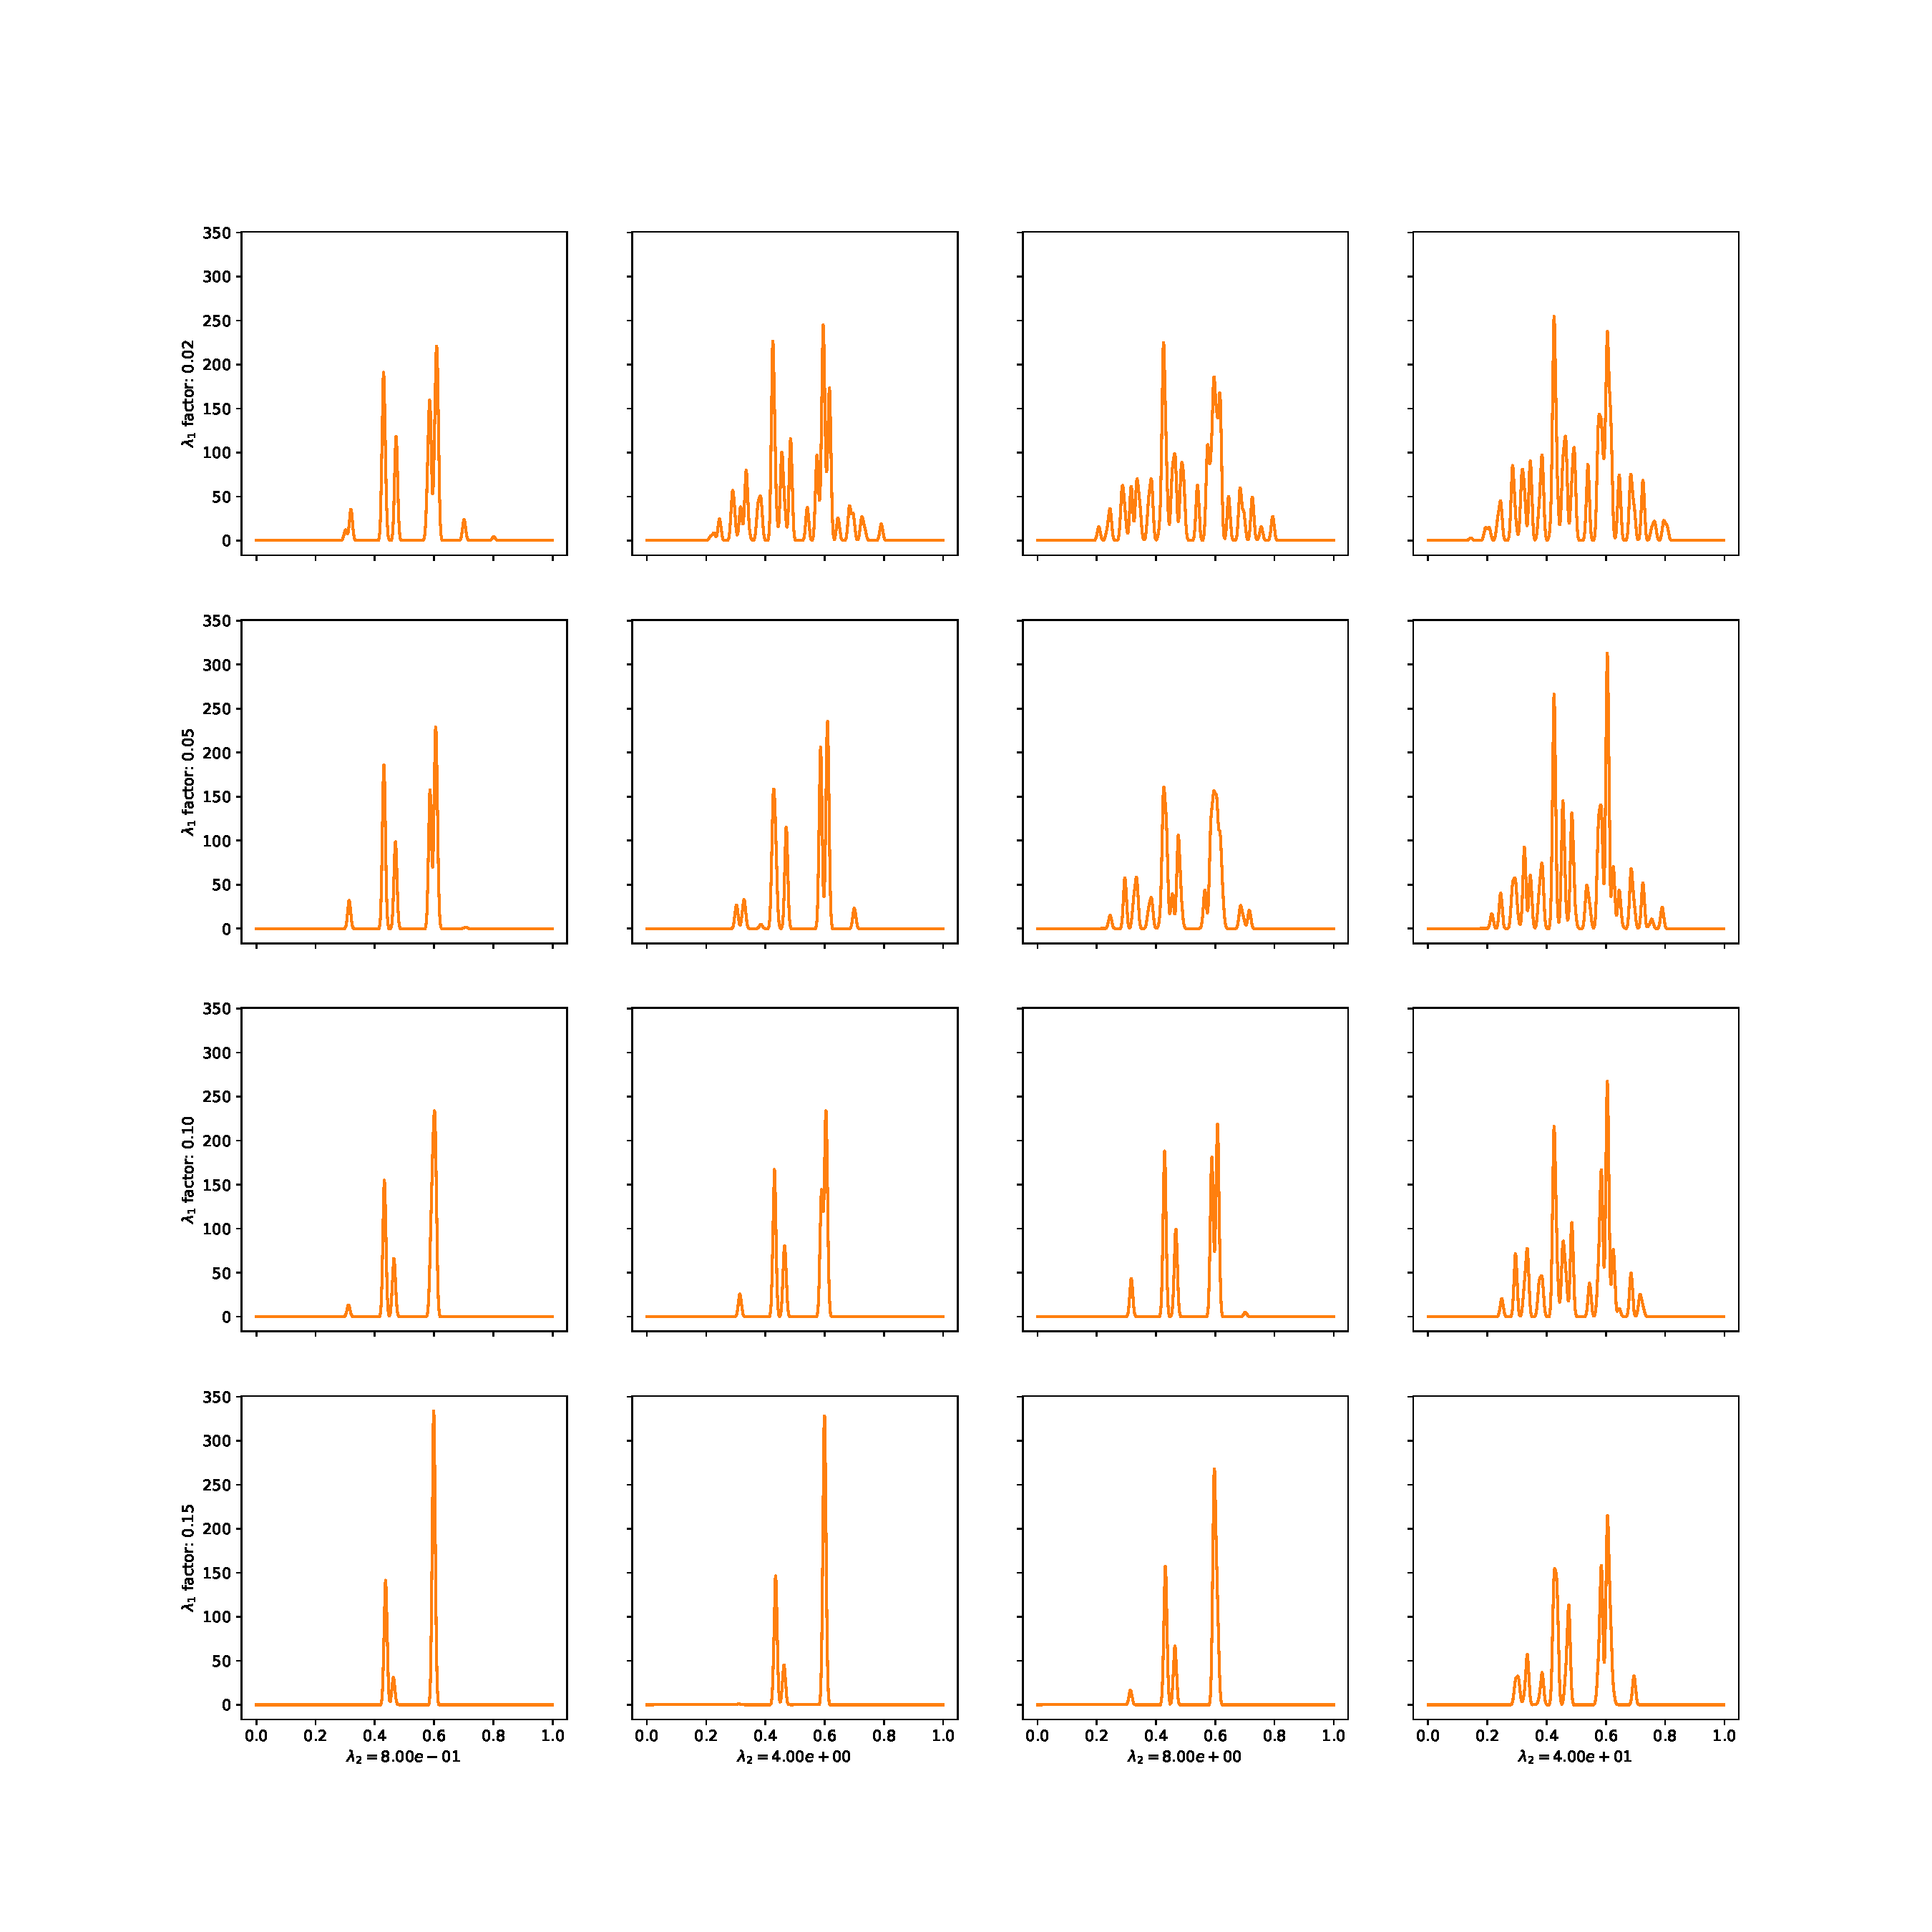
\includegraphics[width=1.2\linewidth]{figures/simple_reco/foreground_merged.pdf}
        \makebox[\textwidth][c]{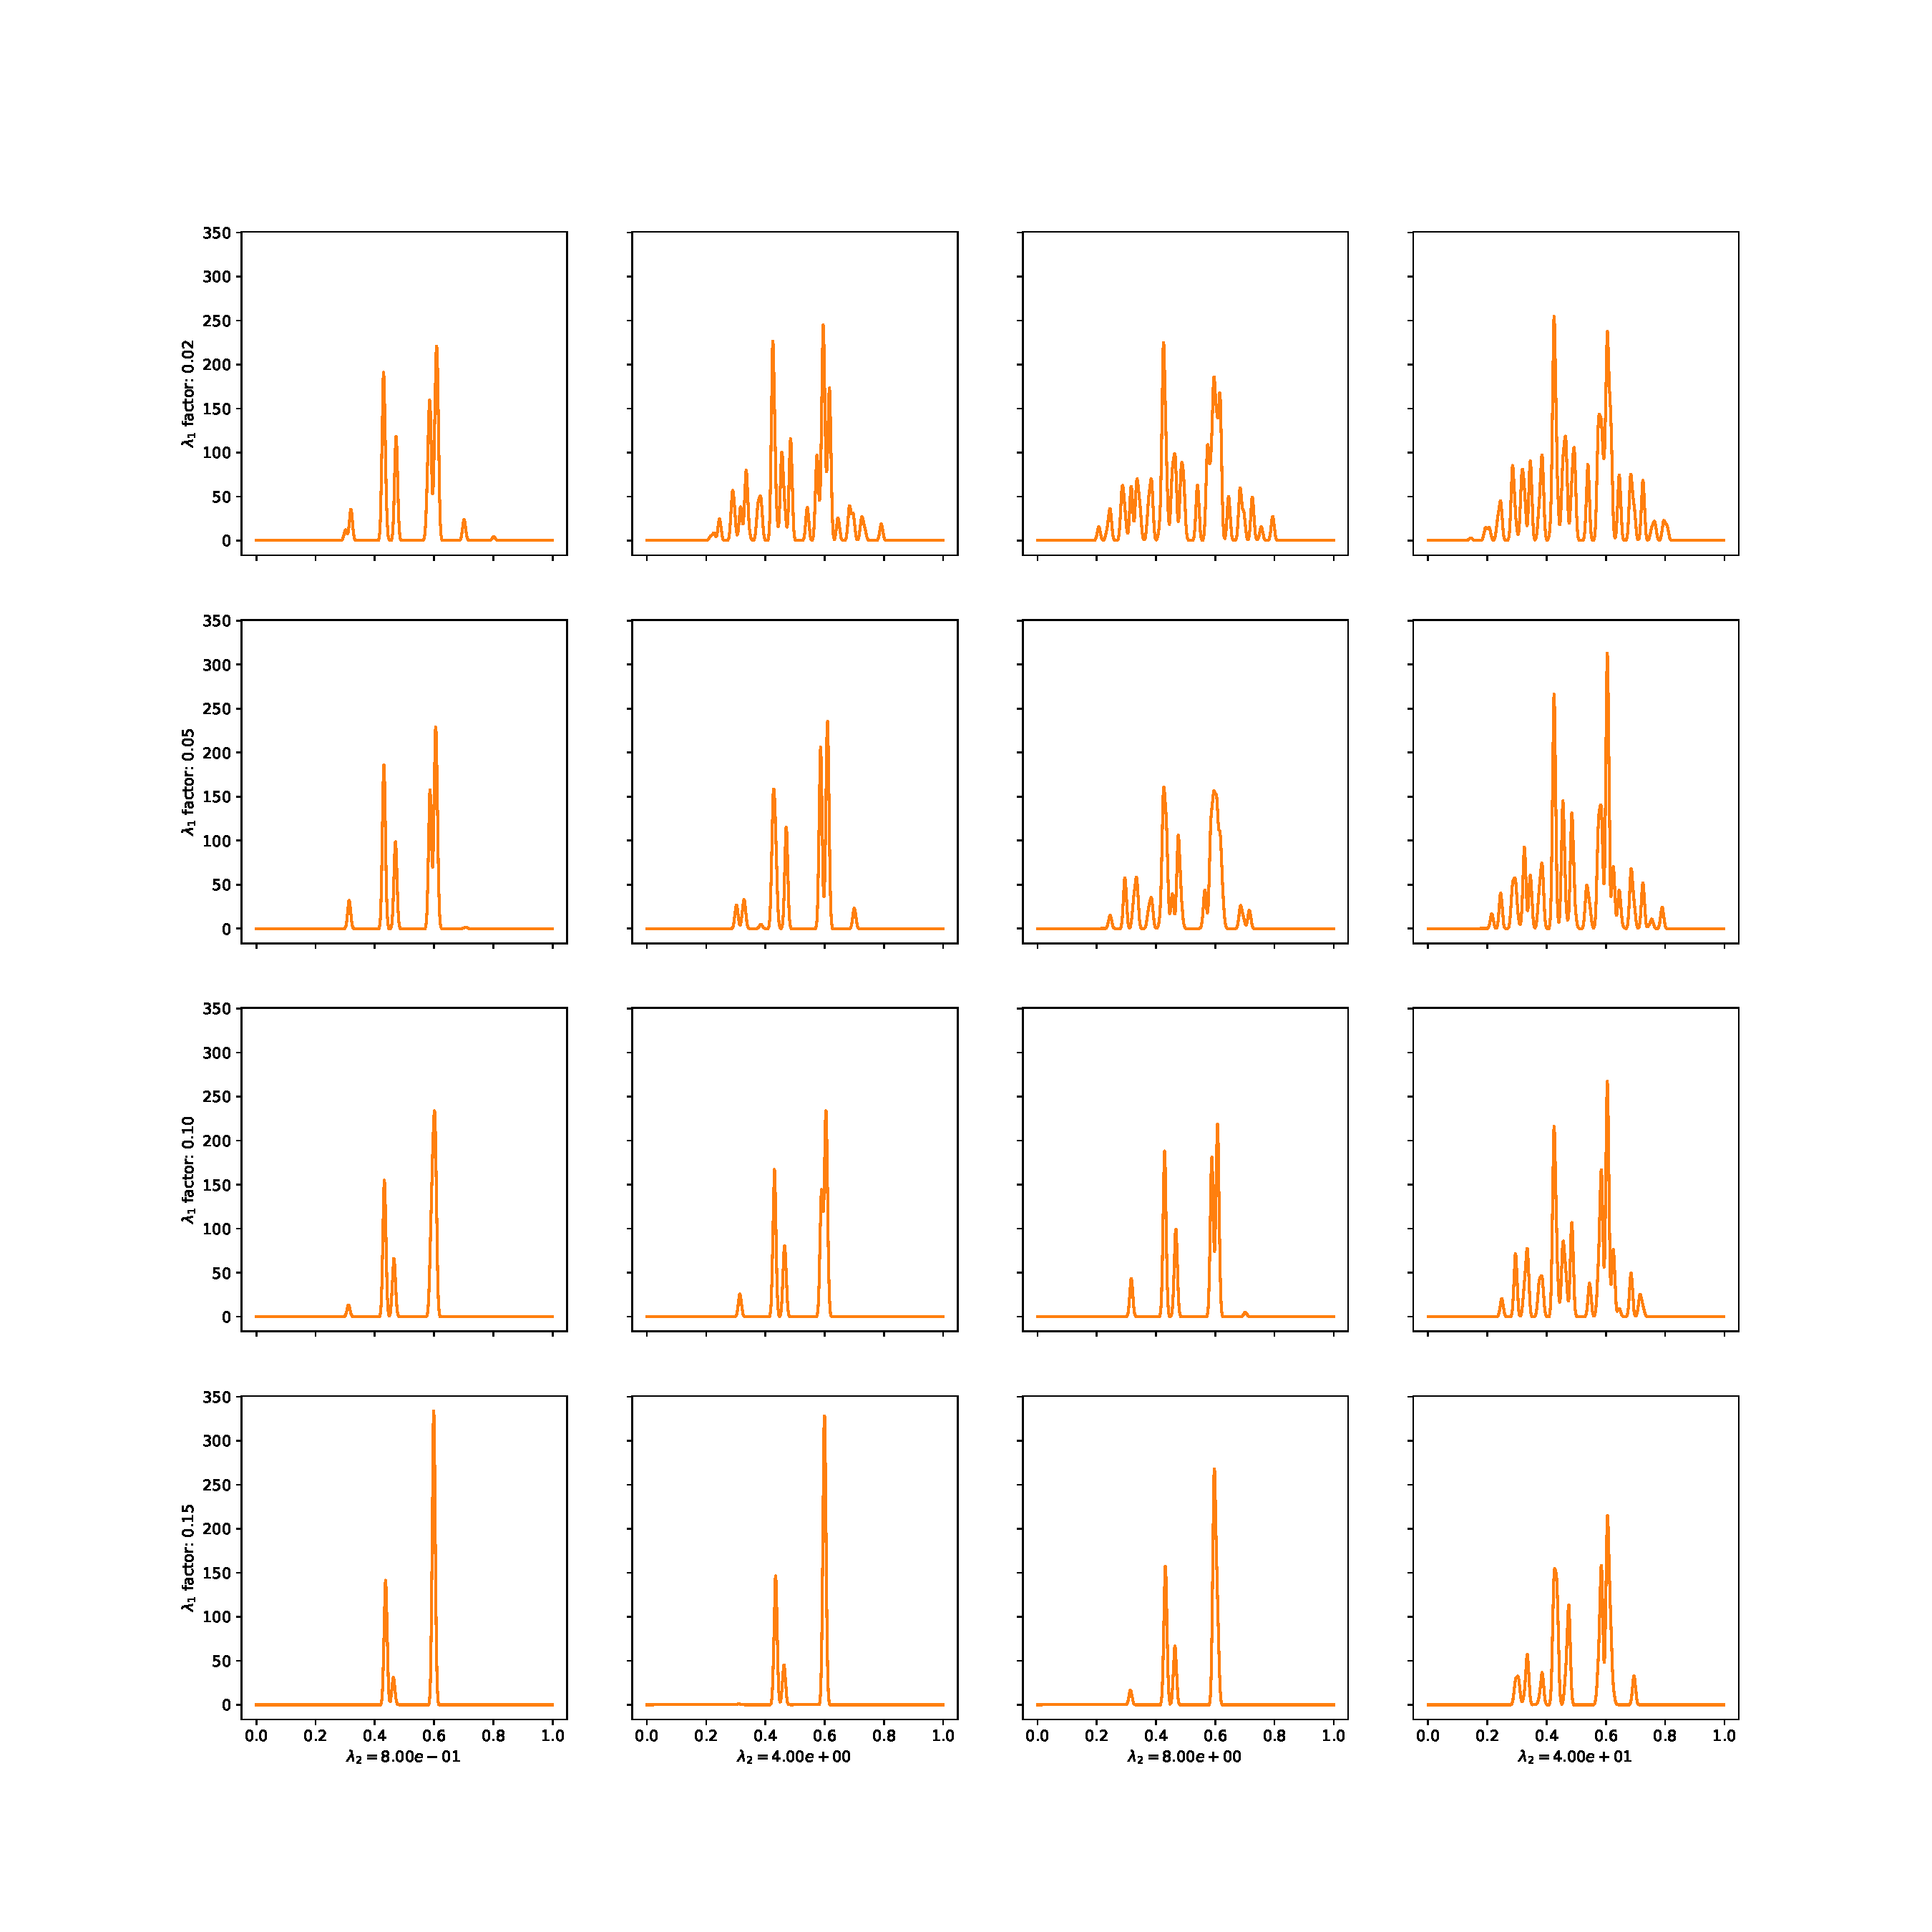
\includegraphics[width=1.1\linewidth, trim=2cm 2.5cm 2cm 3.7cm, clip]{figures/simple_reco/foreground_merged.pdf}}
        \caption{Recovered foreground after convolution with the representation kernel. \textit{Rows :} Increasing value of $\lambda_2$ from top to bottom. \textit{Columns :} Increasing factor $\alpha$ from left to right.}
        \label{fig:simple:fg-merged}        
    \end{figure}

    \vfill

    \begin{figure}[p]
        \makebox[\textwidth][c]{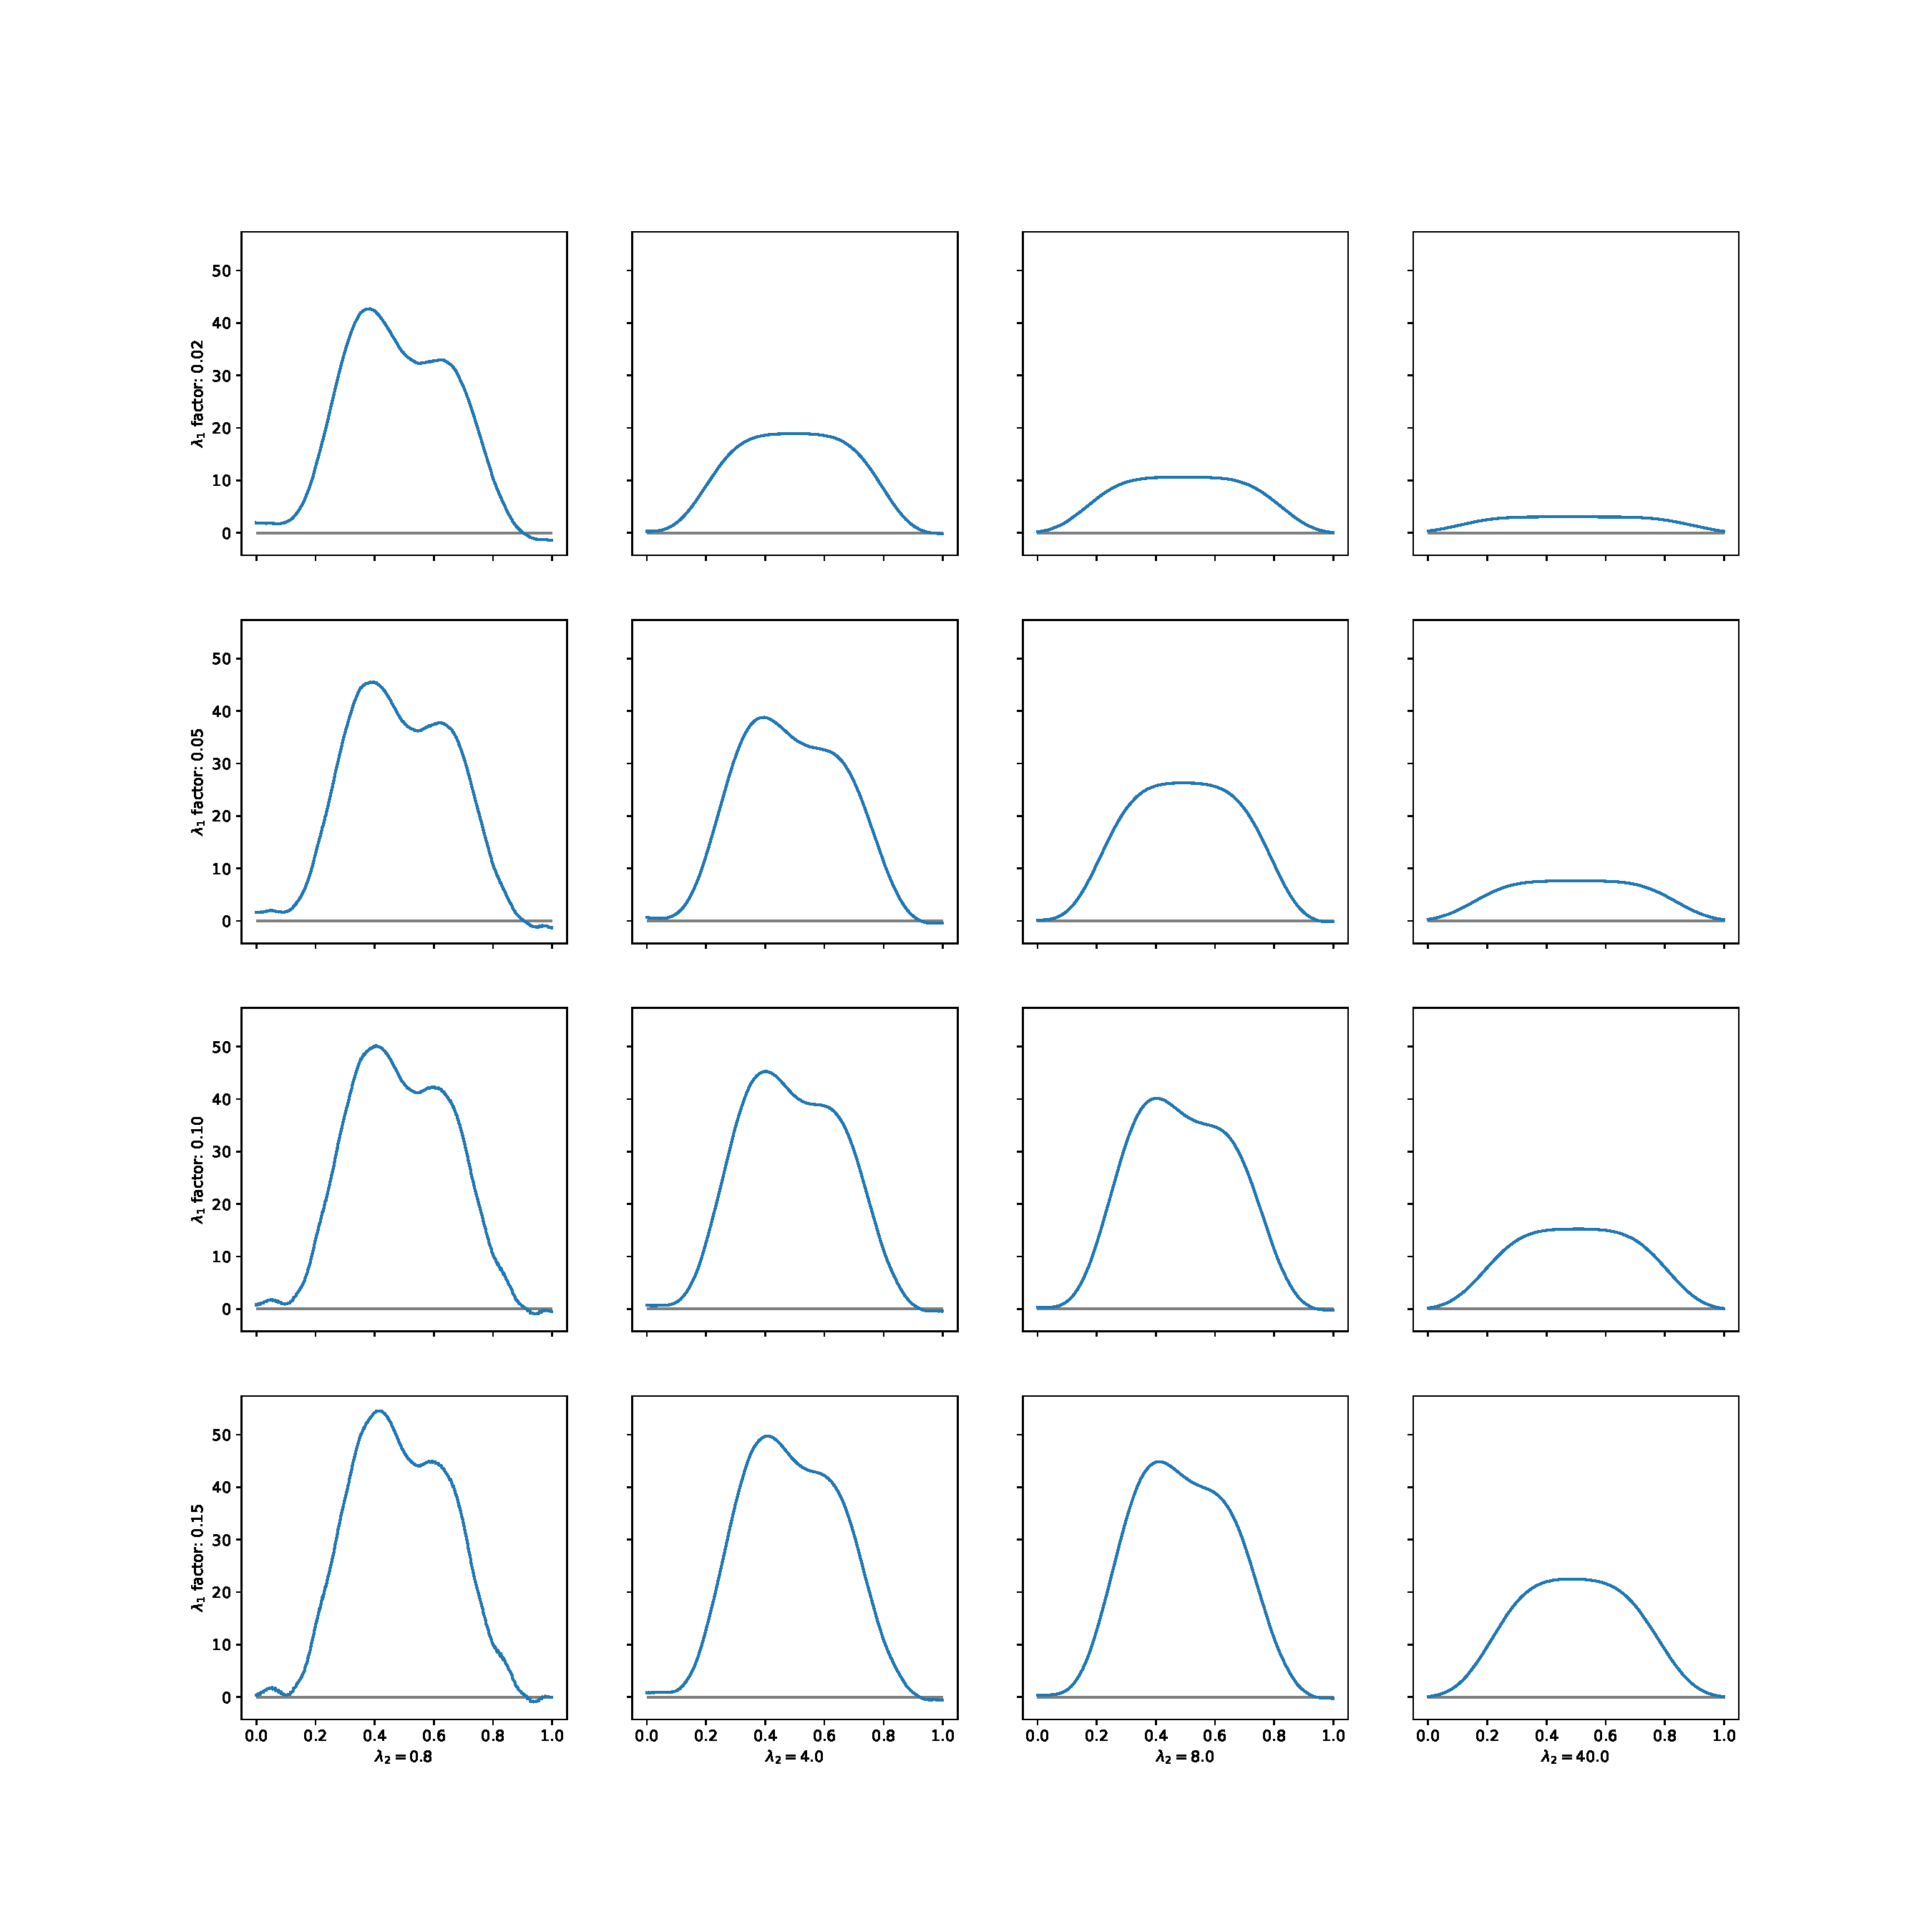
\includegraphics[width=1.1\linewidth, trim=2cm 2.5cm 2cm 3.7cm, clip]{figures/simple_reco/backgrounds.pdf}}
        \caption{Recovered background components, with the same value of regularization parameters as in figure~\ref{fig:simple:fg-merged}.}
        \label{fig:simple:bg}        
    \end{figure}




\clearpage
\section{Calculation for the experiments}
    \label{app:calculation}

    \subsection{Computation of \texorpdfstring{$M_{\lh}$}{M lambda 2}}

    Using the definition of the PSF $g$ in section~\ref{sec:application}, we derive the expression of the matrix $\mathbf{M}_{\lambda_2}$ defined in equation~\eqref{eq:def-Mphi}. For $1\leq k, \ell \leq L$, we have:
    \begin{equation*}
        \mathbf{M}_{\lh}[k, \ell] = \frac{1}{\lh} \left( \langle \phi_k , \phi_\ell \rangle_{\mathcal{H}} + \lh \delta[k - \ell] \right)
    \end{equation*}
    Let us compute the inner product between the functionals $\phi$
    \begin{equation*}
        \begin{aligned}
            \langle \phi_k , \phi_\ell \rangle_{\mathcal{H}} &= \int_\mathcal{X} g(x_k - t) g(x_\ell - t) \mathrm{d}t \\
                &= \int_\mathcal{X} g(- t) g(x_\ell - x_k - t) \mathrm{d}t \\
                &= \int_\mathcal{X} g(t) g(x_\ell - t) \mathrm{d}t \\
                &=  (g * g)(x_\ell - x_k)
        \end{aligned}
    \end{equation*}
    using the symmetry of the kernel $g$ between lines 2 and 3.
    We finally obtain the expression
    \begin{equation*}
        \label{eq:mlambda-1d}
        \mathbf{M}_{\lambda_2}[k, \ell] = \frac{1}{\lh} \left( (g * g)(x_\ell - x_k) + \lh \delta [k - \ell] \right) .
    \end{equation*}

    \subsection{Scaling of \texorpdfstring{$\lh$}{lambda 2}}
    From equation~\eqref{eq:def-Mphi}, the matrix $\mathbf{M}_{\lambda_2}$ can be written as
    \begin{equation}
        \label{eq:mlambda2}
        \mathbf{M}_{\lh} = \mathbf{I}_L +  \frac{1}{\lh}\phih\phih^*
    \end{equation}
    For any vector $\mathbf{h} \in \R^L$, we have
    \begin{align*}
        \forall 1 \leq k \leq L, \quad \left(\phih\phih^*\mathbf{h}\right)[k] &= \sum_\ell \langle \phi_k , \phi_\ell \rangle_{\mathcal{H}} h_\ell \\
            &= \sum_\ell (g * g)(x_\ell - x_k) h_\ell \\
            &= \sum_\ell u_{k - \ell} h_\ell,
    \end{align*}
    with $u_i = (g * g)(x_i)$ for $ \leq i \leq L$. Assuming the support of $\mathbf{h}$ is concentrated in the center of the vector and there is no information near the borders, $\phih\phih^*\mathbf{h}$ can be seen as a convolution between $\mathbf{h}$ and $\mathbf{u}$.

    It is possible to prove that the Lipschitz constant of the operator $\phih\phih^* \in \R^{L \times L}$, which is its maximum singular value, is bounded by $\sqrt{L} \norm{\mathbf{u}}$. Using that $\norm{g*g}_2 = 1$, we can approximate $\norm{\mathbf{u}}_2 \approx \sqrt{L}$ using Riemann sum. Hence, we approximate the maximum singular value of $\phih\phih^*$ with $L$.

    To maintain the term $\frac{1}{\lh} \phih\phih^*$ of the same order as $\mathbf{I}_L$ in $\eqref{eq:mlambda2}$, we set $\lh$ as a ratio of $L$ and we obtain our proposed scaling rule $\lh = \alpha_2 L$.
    


% %%%%%%%%%%%%%%%%%%%%%%%%%%%%%%%%%%%%%%%%%%%%%%
% %%%%%%   FOURRETOUT
% %%%%%%%%%%%%%%%%%%%%%%%%%%%%%%%%%%%%%%%%%%%%%%
% \clearpage    
% \section{Fourretout}

%     \begin{itemize}

%         \item Once we have recognized this fact, we can reuse all the known results for the lasso and apply them in this setting. For instance, uniqueness result for the lasso~\cite{tibshirani2013lasso} or the generalized lasso (if we consider non-invertible operators)~\cite{ali2019generalized} apply to the subproblem. For instance, for large class of sensing matrices $\mathrm{A}$, the transformed $\mathrm{A}$ also has good properties and therefore uniqueness occurs almost surely.
%         \item Same idea: with Fourier measurements and $\Lop_1$ elliptic, if I can include non-invertible operators, I deduce uniqueness results.
        
%         \item Do I do matrices also?
        
%     \end{itemize}

%     \begin{itemize}
%         \item The optimization problem \eqref{eq:hilbertargmin} admits a unique solution given by
%         \begin{equation}
%             \hfh = \Lop^{-1}\Lop^{-1*} \bm{\Phi}^* \left( \bm{\Phi} \Lop^{-1} \Lop^{-1*} \bm{\Phi}^* + \lambda_2 \mathbf{I}_L\right)^{-1} \bm{y}. 
%         \end{equation}
%         \item The optimization problem \eqref{eq:banachargmin} admits at least, and possibly more than, one solution. Moreover, all the solutions share the same measurement vector in the sense that there exists $\bm{y}_{\lambda,\bm{\Phi},\Lop} \in \R^L$ such that 
%         \begin{equation}
%            \forall \hfb \in \mathcal{V}_{\lambda} (\bm{y}, \bm{\Phi} ,\Lop), \quad  \bm{\Phi}(\hfb)  = \bm{y}_{\lambda,\bm{\Phi},\Lop}. 
%         \end{equation}
%     \end{itemize}


%         Fix $\bm{y}$ $\bm{\Phi}$ $\Lop_{\mathcal{B}}$ $\Lop_{\mathcal{H}}$ $\lb$ $\lh$ and set
%     \begin{align}
%         \mathcal{W}_{\lb,\lh} (\bm{y}, \bm{\Phi} ,\Lop_{\mathcal{B}}, \Lop_{\mathcal{H}}) &= \underset{(\fb,\fh) \in \mathcal{B} \times \mathcal{H}}{\arg\min} \| \bm{y} - (\phib (\fb) + \phih (\fh)) \|_2^2  + \lb \| \fb \|_{\mathcal{B}} + \lh \| \fh \|_{\mathcal{H}}^2. 
%     \end{align}    



%     Our main result consists in showing a strong connection between the composite optimization task \eqref{eq:compoargmin} and the two subproblems \eqref{eq:hilbertargmin} and \eqref{eq:banachargmin}. 


%     An inverse problem can be described as follow. We aim at recovering an unknown signal (vector, sequence, function, etc.) from the knowledge of possibly corrupted partial observations. Imagine for instance that you aim at reconstructing an unknown vector $\bm{x}_0 \in \R^N$ from an observation vector $\bm{y} = \mathrm{A} \bm{x}_0 + \epsilon \in \R^M$ where $\mathrm{A} \in \R^{N\times M}$ is a (known) sensing matrix and $\epsilon \in \R^M$ is an i.i.d. Gaussian noise. We assume moreover that $M < N$ such that the system is underdetermined. 

%     The reconstruction task is classically formulated as an optimization problem where the indetermination is overcome by the addition of regularization functional. This leads to optimization problems of the form
%     \begin{equation}
%         \min_{\bm{x}\in \R^N} \| \bm{y} - \mathrm{A} \bm{x} \|_2^2 + \lambda \mathcal{R}( \bm{x} ),
%     \end{equation}
%     where $\mathrm{R}$ is a convex regularization functional which makes the problem well-posed (see below) and $\lambda > 0$ is a parameter balancing the importance of the data-fidelity term $\| \bm{y} - \mathrm{A} \bm{x} \|_2^2$ and the regularization $\mathcal{R}( \bm{x} )$. 

%     Typical choices for the regularization include:
%     \begin{itemize}
%         \item \textbf{Tychonov regularization:} $\mathcal{R}(\bm{x}) = \| \bm{x} \|_2^2$.
        
%         \item \textbf{Sparsity-promoting regularization:}$\mathcal{R}(\bm{x}) = \| \bm{x} \|_1$. In that case, \eqref{eq:} is the well-known LASSO, which is known to promote sparsity and has been extensively studied~\cite{tibshirani1996regression}. In particular, there exists a solution $\widehat{x} \in \R^N$ which is $M$-sparse~\cite{gupta2018continuous}. 
%     \end{itemize}

\bibliographystyle{vancouver}
\bibliography{refs}

\end{document}